\documentclass{article}
%\usepackage{times}
\usepackage{amsmath}
\usepackage{amssymb}
\usepackage{amstext}
%\usepackage[T1]{fontenc}
\usepackage[english]{fp-autoref}
\usepackage{fp-frame}
\usepackage[latin1]{inputenc}
\usepackage{mathpartir}
\usepackage{moreverb}% TEMPORARY
\def\TirName#1{\text{\sc #1}}
\usepackage{stmaryrd}
\usepackage{url}
\usepackage{jbw-arrow}
\usepackage{enumerate}
\usepackage{epsfig}

\newtheorem{condition}{Condition}
\newtheorem{definition}{Definition}
\newtheorem{lemma}{Lemma}

\newcommand{\RT}{\text{RT}}
\newcommand{\RTR}{\RT^R}
\newcommand{\WSMDB}{\text{WS}_{MDB}}
\newcommand{\WSM}{\text{WS}_{M}}
\newcommand{\WS}{\text{WS}}
\newcommand{\says}{\textit{ says }}
\newcommand{\as}{\textit{ as }}
\newcommand{\controls}{\textit{ controls }}
\newcommand{\serves}{\textit{ serves }}
\newcommand{\for}{\textit{ for }}
\newcommand{\carrier}[3]{#1 \textit{ carries } #2 \textit{ for } #3}
\newcommand{\speaksfor}{\Rightarrow}
\renewcommand{\implies}{\supset}
\newcommand{\network}{\mathcal{N}}
\newcommand{\cod}[1]{\llbracket#1\rrbracket}
\newcommand{\subcod}[2]{\llbracket#2\rrbracket_{#1}}
\newcommand{\audit}{\text{audit}}
\newcommand{\aud}{\text{aud}}
\newcommand{\assert}{\text{assert}}
\newcommand{\lookup}{\text{lookup}}
\newcommand{\ok}[1]{\mathit{OK}(#1)}
%\newcommand{\priv}{\ok{T}}
\newcommand{\priv}{\mathbf{priv}}
%\newcommand{\privmdb}{\ok{T_{MDB}}}
\newcommand{\privmdb}{\priv_{MDB}}
\newcommand{\aclmdb}{\acl_{MDB}}
\newcommand{\rawreq}{\mathbf{req}}
\newcommand{\acl}{\mathcal{A}}
\newcommand{\ccl}{\mathcal{C}}
\newcommand{\cclmdb}{\ccl_{MDB}}
\newcommand{\rolecerts}{\mathcal{R}}
\newcommand{\delcerts}{\mathcal{D}}
\newcommand{\keycontrol}{\mathcal{K}}
\newcommand{\true}{\mathbf{true}}
\newcommand{\metaonreq}[1]{\hat{#1}}
\newcommand{\onloc}[2]{#1 \cdot #2}
\newcommand{\onreq}[2]{#1 \cdot #2}
\newcommand{\cloc}{\iota}
\newcommand{\cedge}[1]{\stackrel{#1}{\longleftarrow}}
\newcommand{\cred}[3]{#1 \cedge{#3} #2}
\newcommand{\mathitcred}[3]{\mathit{#1} \cedge{\mathit{#3}} \mathit{#2}}
\newcommand{\expr}{\mathrm{expr}}
\newcommand{\rmem}{\mathrm{rmem}}
\newcommand{\creds}{\mathcal{C}}
\newcommand{\risk}{\kappa}
\newcommand{\risks}{K}
\newcommand{\po}{\preccurlyeq}
\newcommand{\entityrisk}{\mathit{EntityRisk}}
\renewcommand{\implies}{\Rightarrow}
\newcommand{\ents}{\mathrm{ents}}
\newcommand{\credsmean}[1]{\mathcal{S}_{#1}}
\newcommand{\inexprs}{\mathrm{inexprs}}
\newcommand{\bounds}{\mathrm{bounds}}
%\def\twoheadrightarrowfill@{\arrowfill@\relbar\relbar\twoheadrightarrow} 
%\newcommand{\xtwoheadrightarrow}[2][]{\ext@arrow 0359\xtwoheadrightarrowfill@{#1}{#2}} 
\newcommand{\wtedge}[3]{#1 \sarrow{->}{#3} #2}
\newcommand{\xtwoheadrightarrow}[1]{\sarrow{->>}{#1}}
\newcommand{\wtpath}[3]{#1 \xtwoheadrightarrow{#3} #2}
\newcommand{\nodes}[1]{\mathcal{N}_{#1}}
\newcommand{\wtedges}[1]{\mathcal{E}_{#1}}
\newcommand{\graph}[1]{\mathcal{G}_{#1}}
\newcommand{\role}[2]{$\mathit{#1}.\mathit{#2}$}
\newcommand{\CCD}{\textit{GetRisks}}
\newcommand{\checkmem}{\mathrm{checkmem}}
\newcommand{\cesnote}[1]{\textit{(#1 -- c.e.s.)}}

\newcommand{\thmnumbering}{section}
\newtheorem{theorem}{Theorem}[\thmnumbering]
%\newtheorem{definition}{Definition}[\thmnumbering]
\newtheorem{corollary}{Corollary}[\thmnumbering]
\newtheorem{example}{Example}[\thmnumbering]
%\newtheorem{lemma}{Lemma}[\thmnumbering]
%\newtheorem{proposition}{Proposition}[\thmnumbering]
\newenvironment{proof}{\noindent\textit{Proof. }}{\qed\medskip}
%\newcommand{\qed}{$\Box$}
\def\squareforqed{\hbox{\rlap{$\sqcap$}$\sqcup$}}
\def\qed{\ifmmode\squareforqed\else{\unskip\nobreak\hfil
\penalty50\hskip1em\null\nobreak\hfil\squareforqed
\parfillskip=0pt\finalhyphendemerits=0\endgraf}\fi}

\newcommand{\colfigurebox}[5]
{
        \begin{figure}
        \begin{center}
        \framebox[#1]{
                \begin{minipage}{#2}
                \footnotesize
                \vspace{2mm}
                #5
                \vspace{1mm}
                \end{minipage}
                \normalsize
        }
        \caption{#4} 
        \label{#3}
        \end{center}
        \end{figure}
}

\newcommand{\figurebox}[5]
{
        \begin{figure*}
        \begin{center}
        \framebox[#1]{
                \begin{minipage}{#2}
                \footnotesize
                \vspace{2mm}
                #5
                \vspace{1mm}
                \end{minipage}
                \normalsize
        }
        \caption{#4} 
        \label{#3}
        \end{center}
        \end{figure*}
}

%%%%% dduct %%%%%%
\newcommand{\dduct}[2]{
\ensuremath{
\renewcommand{\arraystretch}{1.3}
	\begin{array}[b]{c}
		#1\\\hline
		#2
	\end{array}
\renewcommand{\arraystretch}{1}
}
}
%%%%%%%%%%%%%%%%%%%

\newcommand{\algtab}[1]
{
\vspace*{-3mm}
\begin{tabbing}
\hspace*{12mm}\=\hspace{9mm}\=\hspace{9mm}\=\hspace{6mm}\=\hspace{6mm}\=
\hspace{6mm}\=\\\newcommand{\cmnts}{\noindent\textbf{Comments\hspace{2mm}}}
#1
\end{tabbing}
}
\newcommand{\lt}{\left\{}
\newcommand{\rt}{\right\}}
\newcommand{\Lt}{\left\{\!\!\right.}
\newcommand{\Rt}{\left.\!\!\right\}}
\newcommand{\const}{\mathbf{c}}
\newcommand{\heading}[1]{\noindent\textbf{#1\ \  }}

\newcommand{\schemecomp}[3]{#1\vdash^i#2\preccurlyeq#3}

\newcommand{\Estep}{\rightarrow}
\newcommand{\instance}{\preccurlyeq}
\newcommand{\geninstance}{\trianglelefteq}
\newcommand{\gen}{\mathit{gen}}
\newcommand{\normalize}{\mathit{normalize}}

\newcommand{\iruleone}{\textsc{Sub$^\instance$}}
\newcommand{\iruletwo}{$(\preccurlyeq\!\forall)$}
\newcommand{\irulethree}{$(\forall\!\preccurlyeq)$}

%\newcommand{\seclang}{\lambda_{\text{\rm sec}}}
%\newcommand{\setlang}{\lambda_{\text{\rm set}}}
\newcommand{\pinit}{\ensuremath{p_0}}
%\newcommand{\reduce}{\leadsto}
\newcommand{\reduce}{\rightarrow}
%\newcommand{\eqdefn}{=_{\scriptscriptstyle{\mathit{def}}}}
\newcommand{\subn}{\varphi}
\newcommand{\subndefn}[1]{[#1]}
\newcommand{\restrict}[2]{{#1}\!\mid_{#2}}
\newcommand{\rrow}[2]{\lt \drow{r}{#1}{#2} \rt}
%\newcommand{\refcell}{\mathrm{ref}}
%\newcommand{\tref}{\mathrm{ref}}
%\newcommand{\hmxconfig}[2]{#1/#2}
%\newcommand{\store}{\varsigma}
\newcommand{\rangevec}[3]{#1^{\hspace{4pt}#2 \in \setdefn{1,\ldots,#3}}}
%\newcommand{\initenv}{\Gamma_\iota}
\newcommand{\initenv}{\Delta}
%\newcommand{\extend}[3]{#1\oplus #2 \mapsto #3}
\newcommand{\gdesc}[1]{\text{\textit{#1}}}
\newcommand{\loc}{l}
\newcommand{\setdefn}[1]{\lt#1\rt}
\newcommand{\deref}{\,!}
\newcommand{\assignfn}[1]{{:=}_{#1}}
%\renewcommand{\eabs}[3]{\lambda\langle#1\rangle #2 . #3 }
\newcommand{\credentials}{\mathcal{A}}
\newcommand{\constrain}[2]{#1\!\mid_{#2}}
\newcommand{\remove}[2]{#1\backslash{#2}}
\newcommand{\subrule}{\TirName{Sub}}
\newcommand{\varrule}{\TirName{Var}}
\newcommand{\absrule}{\TirName{Abs}}
\newcommand{\apprule}{\TirName{App}}
\newcommand{\letrule}{\TirName{Let}}
\newcommand{\assignrule}{\TirName{Assign}}
\newcommand{\refrule}{\TirName{Ref}}
\newcommand{\derefrule}{\TirName{Deref}}
\newcommand{\construle}{\TirName{Const}}
\newcommand{\forallelim}{\TirName{$\forall$ Elim}}
\newcommand{\forallintro}{\TirName{$\forall$ Intro}}
\newcommand{\configrule}{\TirName{Config}}
\newcommand{\labinferrule}[3]{\inferrule*[right=\scriptsize#3]{#1}{#2}}
\newcommand{\Labinferrule}[3]{\inferrule*[Right=\scriptsize#3]{#1}{#2}}
\newcommand{\vvec}{\bar{\regv}}
\newcommand{\tvec}{\bar{\tau}}
\newcommand{\existsC}[2]{\exists #1 . #2}
\newcommand{\rename}{\varrho}
\newcommand{\blankheading}[2]
{	
	\vspace{17pt}
	\noindent\textbf{\Large #2}
	\addcontentsline{toc}{#1}{#2}
	\vspace{10pt}
}
\newcommand{\blankchapter}[1]
{	
	\chapter*{#1}
	\addcontentsline{toc}{chapter}{#1}
}
\newcommand{\blanksection}[1]
{	
	\section*{#1}
	\addcontentsline{toc}{section}{#1}
}

%
% ICFP secty definitions
%
\newcommand{\chse}{\ensuremath{\ |\ }}
\newcommand{\chkpriv}[2]{\ensuremath{\mathrm{checkpriv\ }#1\ \mathrm{for\ }#2}}
\newcommand{\inspect}{\ensuremath{\mathrm{inspect}}}
\newcommand{\ite}[3]{\ensuremath{\mathrm{if\ }#1\ \mathrm{then\ }#2\ \mathrm{else\ } #3}}
\newcommand{\nil}{\mathit{nil}}
\newcommand{\fail}{\ensuremath{\mathbf{secfail}}}
\newcommand{\needs}{\ensuremath{\mathrm{\ needs\ }}}
%\newcommand{\fnty}[3]{\ensuremath{#1\rightarrow#2\needs#3}}
\newcommand{\fnty}[3]{\ensuremath{#1\xrightarrow{#3}#2}}
\newcommand{\privs}{\ensuremath{\mathrm{privs}}}
\newcommand{\rmpriv}{\ensuremath{\mathrm{rmpriv}}}
\newcommand{\satisfy}{\ensuremath{\mathit{satisfy}}}
\newcommand{\hsleq}{\ensuremath{\mathit{\preceq_{hs'}}}}
\newcommand{\minsafe}{\ensuremath{\mathit{minsafe}}}
\newcommand{\leastsub}{\ensuremath{\mathit{leastsub}}}
\newcommand{\safesub}{\ensuremath{\mathit{safesub}}}
\newcommand{\vars}{\ensuremath{\mathit{vars}}}
%\newcommand{\pinit}{\ensuremath{p_{\iota}}}
\newcommand{\pset}{\ensuremath{\mathbf{s}}}
\newcommand{\psetinit}{\ensuremath{\pset_{\iota}}}
\newcommand{\cons}[2]{\ensuremath{#1\!::\!#2}}
\newcommand{\constr}{\ensuremath{\ /\ }}
\newcommand{\stack}{\ensuremath{\mathtt{S}}}
%\newcommand{\stack}{\ensuremath{\mathbf{s}}}
\newcommand{\gpset}{\ensuremath{R}}
%\newcommand{\subn}{\ensuremath{S}}
\newcommand{\vsubn}{\ensuremath{\hat{S}}}
\newcommand{\isecty}{\ensuremath{\mathit{isecty}}}
\newcommand{\mt}{\ensuremath{\mathit{mt_{\scriptscriptstyle{\tpc}}}}}
%\newcommand{\mt}{\ensuremath{\mathit{mt}}}
\newcommand{\MT}{\ensuremath{\mathit{MT}}}
\newcommand{\MTfn}{\ensuremath{f}}
\newcommand{\dom}{\ensuremath{\mathit{Dom}}}
\newcommand{\var}{\ensuremath{\mathit{Vars}}}
\newcommand{\sectyfail}{\ensuremath{\mathbf{sectyfail}}}
\newcommand{\infsecty}{\ensuremath{\mathit{infer\_secty}}}
\newcommand{\sconstrs}{\ensuremath{\mathit{scs}}}
\newcommand{\tpc}{\ensuremath{\mathit{TPC}}}
\newcommand{\pc}{\ensuremath{\mathit{PC}}}
\newcommand{\tc}{\ensuremath{\mathit{TC}}}
\newcommand{\close}{\ensuremath{\mathit{close}}}
\newcommand{\verify}{\ensuremath{\mathit{verify}}}
\newcommand{\glb}{\ensuremath{\mathit{glb}}}
\newcommand{\istack}{\ensuremath{\stack_{\iota}}}
\newcommand{\stackinit}{\ensuremath{\stack_{\iota}}}
%\newcommand{\mapping}[2]{#1 \triangleright #2}
\newcommand{\mapping}[2]{[#2/#1]}
\newcommand{\stackframe}[3]{\langle #1, #2, #3 \rangle}
\newcommand{\constack}[4]{\ensuremath{\stackframe{#1}{#2}{#3}\hspace{-2pt} :: \! #4}}
\newcommand{\revstack}[4]{\ensuremath{#4 @ \stackframe{#1}{#2}{#3}}}
%\newcommand{\signedfn}[3]{\ensuremath{{}^{#3}\!\lambda #1.#2}}
\newcommand{\signedfn}[3]{\ensuremath{\lambda #1.#2.#3}}
%\newcommand{\signedfn}[3]{\ensuremath{\lambda\, #1.#2 \rhd #3}}
\newcommand{\access}{\ensuremath{\credentials}}
%\newcommand{\enabled}{\ensuremath{\mathcal{F}}}
\newcommand{\enabled}{\pset}
%\newcommand{\secderv}{\ensuremath{\vdash_{\!\scriptscriptstyle{\access}}}}
\newcommand{\secderv}{\ensuremath{\vdash}}
\newcommand{\secvar}{\ensuremath{\alpha}}
\newcommand{\secty}{\ensuremath{\tau}}
\newcommand{\lp}{\ensuremath{\mathit{lp}}}
%\newcommand{\seclang}{\ensuremath{\lambda_{\text{sec}}}}
\newcommand{\unit}{\ensuremath{\text{unit}}}
\newcommand{\Let}{\ensuremath{\mathrm{\ let\ }}}
\newcommand{\In}{\ensuremath{\mathrm{\ in\ }}}
\newcommand{\translt}{\TirName{trans$\le$}}
\newcommand{\reflt}{\TirName{ref$\le$}}
\newcommand{\sub}{\TirName{sub}}
\newcommand{\subtr}{\TirName{sub}}
\newcommand{\vartr}{\TirName{var}}
\newcommand{\fntr}{\TirName{abs}}
\newcommand{\appltr}{\TirName{app}}
\newcommand{\lptr}{\RuleLetPrivYes}
\newcommand{\lpftr}{\RuleLetPrivNo}
\newcommand{\cptr}{\RuleCheckPriv}
\newcommand{\fnlt}{$\rightarrow\le$}
\newcommand{\inlt}{\TirName{coerce$\le$}}
\newcommand{\psvar}{\ensuremath{\rho}}
\newcommand{\tysubn}{\ensuremath{\Theta}}
\newcommand{\soln}[1]{\ensuremath{\lfloor#1\rfloor}}
\newcommand{\exf}[1]{\ensuremath{\mathit{#1}}}
\newcommand{\fullvers}[1]{}
\newcommand{\shortvers}[1]{#1}
\newcommand{\slredex}[2]{#1,#2}
\newcommand{\false}{\text{\bf false}}
\newcommand{\jdirect}[6]{#1, #2, #3, #4 \vdash #5 : #6}

\def\snote#1{\ \ [[\ \ \textbf{#1}\ \ ]]\ \ }

%
% ECOOP capty definitions
%
%\newcommand{\gdesc}[1]{\text{\textit{#1}}}
\newcommand{\idworld}{\mathit{ID}}
\newcommand{\idset}{}
\newcommand{\lab}{d}
\newcommand{\labset}{D}
\newcommand{\Alabworld}{\mathcal{L}_a}
\newcommand{\Blabworld}{\mathcal{L}_b}
\newcommand{\labworld}{\mathcal{D}}
\newcommand{\intface}{\iota}
\newcommand{\uintface}{\varphi}
\newcommand{\coreobj}[1]{[#1]}
\newcommand{\objdefn}[3]{\coreobj{#1}\cdot #2 \cdot #3}
\newcommand{\varobjdefn}[3]{#1\cdot #2 \cdot #3}
\newcommand{\recdefn}[1]{\{ #1 \}}
\newcommand{\recgen}[1]{{\pi}_{#1}}
%\newcommand{\setdefn}[1]{\recdefn{#1}}
%\newcommand{\capab}[2]{\langle #1,#2 \rangle}
%\newcommand{\capab}[3]{\objdefn{#1}{#2}{#3}}
%\newcommand{\itranslate}[1]{\mathit{trans}\ #1}
\newcommand{\itranslate}[1]{\hat{#1}}
\newcommand{\itranslatewide}[1]{\widehat{#1}}
%\newcommand{\stranslate}[1]{\hat{#1}}
\newcommand{\stranslate}[1]{#1}
\newcommand{\itrans}[1]{\itranslate{#1}}
\newcommand{\strans}[1]{\stranslate{#1}}
\newcommand{\itranswide}[1]{\widehat{#1}}
\newcommand{\stranswide}[1]{#1}
%\newcommand{\project}[2]{#1/#2}
%\newcommand{\modify}[3]{#1[#2 = #3]}
%\newcommand{\elevate}[1]{[#1]}
%\newcommand{\rowabbrv}[1]{[#1]}
\newcommand{\project}[2]{#1.#2}
\newcommand{\modify}[3]{#1\{#2 = #3\}}
\newcommand{\elevate}[1]{\{#1\}}
\newcommand{\rowabbrv}[1]{\{#1\}}
\newcommand{\memcheck}[2]{#2\ni#1}
\newcommand{\notmemcheck}[2]{#2\not\ni#1}
\newcommand{\memcheckprim}[1]{\ni_{#1}}
\newcommand{\projprim}[1]{/_{#1}}
%\newcommand{\methlist}{\mathit{ml}}
\newcommand{\methlist}{\varrho}
%\newcommand{\loc}{l}
\newcommand{\send}[3]{#1.#2(#3)}
\newcommand{\select}[2]{#1.#2}
%\newcommand{\store}{\sigma}
\newcommand{\config}[3]{#1,#2,#3}
\newcommand{\isoopconfig}[2]{#1/#2}
\newcommand{\hmxconfig}[2]{#1,#2}
%\newcommand{\ocap}{\ensuremath{o_{\mathrm{cap}}}}
\newcommand{\ocap}{\ensuremath{\mathrm{pop}}}
%\newcommand{\isoop}{\ensuremath{\mathrm{isoop}_{\mathrm{set}}}}
\newcommand{\isoop}{\ensuremath{\mathrm{isoop}}}
%\newcommand{\projml}{\ensuremath{P\!\Lambda_{\mathrm{ref}}}}
\newcommand{\projml}{\ensuremath{\mathrm{pml}_{\scriptstyle{B}}}}
%\newcommand{\reduce}{\rightarrow}
%\newcommand{\extend}[3]{#1\!\parallel\! #2 \mapsto #3}
%\newcommand{\extend}[3]{#1\!\oplus\! #2 \mapsto #3}
\newcommand{\extend}[3]{#1[#2 \mapsto #3]}
\newcommand{\meths}[1]{\text{\rm meths}(#1)}
\newcommand{\ivars}[1]{\text{\rm ivars}(#1)}
\newcommand{\ifacevars}[1]{\text{\rm vars}_{\intface}(#1)}
%\newcommand{\hole}{\text{\vbox{\hrule height 0.015cm width 0.15cm}}}
%\newcommand{\fv}[1]{\text{\rm fv}(#1)}
%\newcommand{\domain}[1]{\text{\rm dom}(#1)}
\newcommand{\snks}[1]{\text{\rm usr}(#1)}
\newcommand{\obj}[2]{\text{\rm obj}_{#1}(#2)}
%\newcommand{\cast}[2]{(#1)#2}
%\newcommand{\cast}[2]{\llcorner\!#2\!\lrcorner_{#1}}
%\newcommand{\cast}[3]{#1\!\shortmid\!_{\!\scriptscriptstyle{#2}}{#3}}
\newcommand{\cast}[3]{#1\!\shortmid\!(#2,#3)}
\newcommand{\multicast}[2]{#1\!\shortmid\!#2}
%\newcommand{\elet}[3]{\mathrm{let}\,#1=#2\,\mathrm{in}\,#3}
%\newcommand{\etestprim}[1]{\mathord{?}_{#1}}
%\newcommand{\eaccess}[2]{#1.#2}
%\newcommand{\eaccessprim}[1]{._{#1}}
\newcommand{\refcell}{\text{\rm ref}}
\newcommand{\successor}{\text{\rm succ}}
\newcommand{\pred}{\text{\rm pred}}
\newcommand{\iszero}{\text{\rm zero}}
\newcommand{\olab}{\text{\rm obj}}
\newcommand{\weaklab}{\text{\rm strong}}
\newcommand{\snkslab}{\text{\rm usr}}
\newcommand{\srclab}{\text{\rm src}}
\newcommand{\intfacelab}{\text{\rm ifc}}
\newcommand{\setlab}{\text{\rm set}}
\newcommand{\getlab}{\text{\rm get}}
\newcommand{\deletelab}{\text{\rm delete}}
\newcommand{\readlab}{\text{\rm read}}
\newcommand{\writelab}{\text{\rm write}}
\newcommand{\subsetfn}{\text{\rm subseteq}}
\newcommand{\castfn}{\text{\rm cast}}
\newcommand{\upcastfn}{\text{\rm upcast}}
\newcommand{\caprec}[2]{\recdefn{\olab = #1, \intfacelab = #2}}
%\newcommand{\credentials}{\mathcal{A}}
\newcommand{\vpre}{\tpre}
\newcommand{\vabs}{\tabs}
%\newcommand{\defeq}{=_{\scriptscriptstyle{\mathrm{def}}}}
%\newcommand{\defeq}{\stackrel{\mathrm{def}}{=}}
\newcommand{\defeq}{\triangleq}
\newcommand{\bisimilar}{\simeq}
\newcommand{\redexsimilar}{\approxeq}
\newcommand{\contextsimilar}{\approxeq}
%\renewcommand{\tset}[1]{[#1]}
%\renewcommand{\ourX}{\ensuremath{\mathrm{ROWS}}}
\newcommand{\tref}{\refcell}
\newcommand{\ycomb}{Y}
%\newcommand{\self}{\varsigma}
\newcommand{\ivar}{i}
%\newcommand{\initenv}{\Gamma_1}
%\newcommand{\objt}[2]{#1\ \mathbf{withface}\ #2}
\newcommand{\prettyrow}[1]{[#1]}
%\newcommand{\objt}[2]{#1\ \cdot\ #2}
\newcommand{\objt}[3]{{#1}^{#2}_{#3}}
%\newcommand{\objt}[3]{{#1}\cdot{#2}-{#3}}
\newcommand{\intt}{\mathrm{int}}
\newcommand{\objintt}{\mathbf{int}}
\newcommand{\unitt}{\mathrm{unit}}
\newcommand{\labinit}{\lab_1}
%\newcommand{\schemecomp}[3]{#1\vdash^i#2\preccurlyeq#3}
%\newcommand{\jocap}[5]{#1,#2,#3\vdash#4 : #5}
\newcommand{\jocap}[5]{#1,#3\vdash#4 : #5}
\newcommand{\assume}{\Gamma}
%\newcommand{\vecdefn}[3]{#1^{\hspace{6pt}#2 \in \setdefn{1,\ldots,#3}}}
\newcommand{\vecdefn}[3]{{#1}^{\hspace{4pt}0<{#2}\le{#3}}}
%\newcommand{\methods}[2]{#1^{\hspace{6pt}#2}}
\newcommand{\codt}[1]{\llparenthesis\,#1\,\rrparenthesis}
\newcommand{\codtin}[1]{\llparenthesis\,#1\,\rrparenthesis_{\tin}}
\newcommand{\codtout}[1]{\llparenthesis\,#1\,\rrparenthesis_{\tout}}
\newcommand{\invcodt}[1]{\rrparenthesis#1\llparenthesis}
\newcommand{\fndestruct}[3]{#1;\ #2 \mapsto #3}
\newcommand{\ksset}[1]{{\text{\emph{Set}}}_{#1}}
\newcommand{\kmeth}[1]{{\text{\emph{Meth}}}_{#1}}
\newcommand{\kifc}[1]{{\text{\emph{Ifc}}}_{#1}}
%\newcommand{\weaken}[3]{\mathbf{weak}(#1,#2,#3)}
\newcommand{\weaken}[2]{\mathbf{weak}_{#2}(#1)}
%\newcommand{\eabs}[2]{\lambda#1.#2}
\newcommand{\cellobj}[2]{#1 \cdot #2}
\newcommand{\newcell}[2]{\refcell_{#1}#2}
\newcommand{\unitv}{()}
\newcommand{\cget}[1]{\send{#1}{\getlab}{}}
\newcommand{\cset}[2]{\send{#1}{\setlab}{#2}}
\newcommand{\intersect}[2]{#1\wedge#2}
\newcommand{\union}[2]{#1\vee#2}
\newcommand{\unionprim}[1]{\vee_{#1}}
\newcommand{\difference}[2]{#1\ominus#2}
\newcommand{\diffprim}[1]{\ominus_{\!#1}}
\newcommand{\differenceprim}[1]{\ominus_{#1}}
\newcommand{\reduceisect}{\reduce_\wedge}
%\newcommand{\existsC}[2]{\exists#1.#2}
\newcommand{\noneset}{\varnothing}
\newcommand{\allset}{\coset{\noneset}}
\newcommand{\addmem}[2]{#1{\scriptstyle\oplus}#2}
\newcommand{\removemem}[2]{#1{\scriptstyle\ominus}#2}
\newcommand{\setmeaning}[1]{\langle#1\rangle}
%\newcommand{\tin}{\cdot}
%\newcommand{\tout}{-}
\newcommand{\tin}{+}
\newcommand{\tout}{-}
\newcommand{\ttop}{\top}
\newcommand{\tbot}{\bot}
\newcommand{\setv}{\rowv}
\newcommand{\allsett}{\omega}
\newcommand{\nonesett}{\varnothing}
%\newcommand{\fielduk}[2]{\stackrel{\;#2}{#1}}
\newcommand{\fielduk}[2]{#1#2}
\newcommand{\fieldint}[1]{\fielduk{#1}{\tin}}
\newcommand{\fieldoutt}[1]{\fielduk{#1}{\tout}}
%\newcommand{\fieldint}[1]{\dot{#1}}
%\newcommand{\fieldoutt}[1]{\bar{#1}}
\newcommand{\kcon}{\text{\emph{Con}}}
\newcommand{\compoundC}{\mathbf{C}}
\newcommand{\srow}[3]{\fielduk{#1}{#2},#3}
\newcommand{\snext}{,}
\newcommand{\sys}{\ensuremath{\system{1}{=}}}
\newcommand{\inlong}[1]{#1}
\newcommand{\labs}[2]{\lambda #1 . #2}
\newcommand{\tyinf}{\ensuremath{\mathit{infer}}}
\newcommand{\unify}{\ensuremath{\mathit{unify}}}
\newcommand{\kprow}[1]{{\text{\emph{Prow}}}_{#1}}
\newcommand{\rurow}[2]{\tset{\unionrow{\fielduk{r}{#1}}{#2}}}
\newcommand{\simplify}{\ensuremath{\mathit{simplify}}}
\newcommand{\confusion}{\ensuremath{\mathit{confusion}}}
%\newcommand{\close}{\ensuremath{\mathit{close}}}
\newcommand{\ctrans}{\ensuremath{\mathit{Trans}}}
\newcommand{\ctransp}{\ensuremath{\mathit{Trans_{row}}}}
\newcommand{\cfn}{\ensuremath{\mathit{Fn}}}
\newcommand{\crow}{\ensuremath{\mathit{Row}}}
%\newcommand{\tyinf}{\ensuremath{\mathit{infer}}}
\newcommand{\absrow}{\partial\tabs}
\newcommand{\groundrow}{\varrho}
%\newcommand{\fail}{\mathbf{fail}}
\newcommand{\fieldel}{\mathit{f}}
\newcommand{\rowsplit}{\mathit{split}}
\newcommand{\multivar}{\ensuremath{\gamma}}
\newcommand{\extnsn}{\varepsilon}
\newcommand{\compsubn}{\vartheta}
\newcommand{\privset}{\mathcal{R}}
\newcommand{\mvar}{\mu\nu}
\newcommand{\abrvrow}{ar}
\newcommand{\arow}[3]{\langle #1, #2, #3 \rangle}
\newcommand{\smid}{\!\shortmid\!}
%\newcommand{\range}{\mathrm{rng}}
\newcommand{\fuse}{\mathit{fuse}}
\newcommand{\prow}{\pi}
\newcommand{\emptyprow}{\epsilon}
\newcommand{\urset}{\mathcal{R}}
\newcommand{\unionrow}[2]{#1\ltimes#2}
\newcommand{\cprow}[2]{#1\smid#2}
\newcommand{\prowt}{\pi}
\newcommand{\rawform}[4]{(\unionrow{#1}{\cprow{#2}{#3}}\snext #4)}
\newcommand{\tground}{\hat{\tau}}
\newcommand{\nat}{\mathbb{N}}
\newcommand{\pair}[2]{#1 * #2}
\newcommand{\coset}[1]{\bar{#1}}
%\newcommand{\stacked}[1]{\lfloor#1\rfloor}
\newcommand{\stacked}[1]{\cdot#1\cdot}
\newcommand{\venv}{\gamma}
\newcommand{\closure}[2]{\mathtt{C}({#1},{#2})}
\newcommand{\onflag}[1]{\mathbf{on}(#1)}
\newcommand{\offlag}{\mathbf{off}}
\newcommand{\shadow}[2]{#1 ; #2}
\newcommand{\flagsym}{\mathbf{f}}
\newcommand{\gleanenv}{\mathrm{env}}
\newcommand{\valueworld}{\mathbb{V}}
\newcommand{\OK}{\mathit{ok}}
\newcommand{\tOK}{\tau_{\OK}}
\newcommand{\tdead}{\tau_{dp}}
\newcommand{\upddef}{\triangleright}
\newcommand{\defupd}[2]{#1 \upddef #2}
\newcommand{\tsetp}[1]{\tset{\cdot#1\cdot}}
\newcommand{\inject}[1]{{}^\backprime#1}
\newcommand{\match}[3]{\text{\rm match}\ #1\ \text{\rm{with}}\ #2 \rightarrow #3}
\newcommand{\defuser}{\partial}
\newcommand{\defmatch}[1]{\hole \rightarrow #1}
\newcommand{\scod}[1]{\codp{#1}{}}
\newcommand{\succeedmacro}{\text{\bf succeed}}
\newcommand{\failmacro}{\text{\bf fail}}
\newcommand{\freshlab}[1]{\text{\bf{fresh}}_{#1}()}
\newcommand{\sframe}{\mathit{f}}
\newcommand{\oldest}{\text{\rm oldest}}
\newcommand{\sectrans}{$\seclang$-to-$\projml$}
\newcommand{\vb}[1]{\texttt{#1}}
\newcommand{\public}{\text{\texttt{public}}}
\newcommand{\private}{\text{\texttt{private}}}
%\renewcommand{\protected}{\text{\texttt{protected}}}
\newcommand{\metaj}{\mathcal{J}}
\newcommand{\locrule}{\TirName{Loc}}
\newcommand{\eassign}[2]{\mathord{:=}\,#1\,#2}
\newcommand{\eass}[1]{\mathord{:=}\,#1}
\newcommand{\vcod}[1]{\langle#1\rangle}
\newcommand{\rcodp}[2]{\langle#1\rangle_{#2}}
\newcommand{\weakface}[2]{#1\backslash_{#2}}
\newcommand{\labstack}{\delta}
\newcommand{\labcons}[2]{#1::#2}
\newcommand{\rev}{\mathrm{rev}}
\newcommand{\codconfig}[3]{\codp{\hmxconfig{#1}{#2}}{#3}}
\newcommand{\codsim}{\lhd}
\newcommand{\oreduce}{\hookrightarrow}
\newcommand{\Ehole}{[\,]}
\newcommand{\selfobj}[1]{[#1]}
\newcommand{\selft}[1]{\prettyrow{#1}}
\newcommand{\eseclang}{\seclang^{\stack}}
\newcommand{\codE}[3]{\cod{(#2, #3, #1)}}
\newcommand{\slreduce}{\reduce}
\newcommand{\frun}{f_{\mathrm{run}}}
\newcommand{\silenturl}[1]{}
\newcommand{\eg}{e.g.~}
\newcommand{\linfer}[3]{\inferrule*[right=\textsc{\scriptsize#3}]{#1}{#2}}

%
% DANGEROUS REDEFINES!
%
%\renewcommand{\drow}[3]{\fielduk{#1}{#2},#3}
%\renewcommand{\tpre}{\tin}
%\renewcommand{\tabs}{\tout}






\newcommand{\tmstructfig}
{
\begin{fpfig}[t]{Structure of an Authorization Decision}{figure-tmstruct}
\vspace{2mm}
\begin{tabular}{cc}
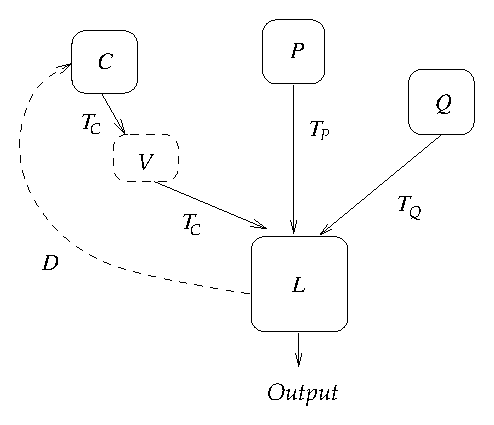
\includegraphics{tmstruct}
& 
\hspace{-10mm}
$
\begin{array}[b]{rcl}
P &:& \text{Policy}\\
C &:& \text{Certificates}\\
Q &:& \text{Authorization Query}\\
V &:& \text{Certificate Validation}\\
L &:& \text{Authorization Mechanism}\\
T_P &:& \text{Policy Compilation}\\
T_C &:& \text{Credential Encoding}\\
T_Q &:& \text{Query Compilation}\\
D &:& \text{Distributed Certificate Discovery}\\
\end{array}
$
\end{tabular}
\vspace{2mm}
\end{fpfig}
}


\newcommand{\BANrulesfig}
{
\begin{fpfig}[t]{Some Inference Rules of BAN Logic}{figure-BANrules}
\begin{mathpar}
\inferrule[message-meaning-1]
  { P \mkeyword{believes} (P \stackrel{K}{\longleftrightarrow} Q) \\
    P \mkeyword{sees} \{X\}_K }
  { P \mkeyword{believes} (Q \mkeyword{said} X) }

\inferrule[message-meaning-2]
  { P \mkeyword{believes} (\stackrel{K}{\longmapsto} Q) \\
    P \mkeyword{sees} \{X\}_{K^{-1}} }
  { P \mkeyword{believes} (Q \mkeyword{said} X) }

\inferrule[jurisdiction]
  { P \mkeyword{believes} (Q \mkeyword{controls} X) \\
    P \mkeyword{believes} (Q \mkeyword{believes} X) }
  { P \mkeyword{believes} X }

\inferrule[signature-check]
  { P \mkeyword{believes} (\stackrel{K}{\longmapsto} Q) \\
    P \mkeyword{sees} \{X\}_{K^{-1}} }
  { P \mkeyword{sees} X }
%\inferrule[nonce-verification]
%  { P \mkeyword{believes} \keyword{fresh}(X) \\
%    P \mkeyword{believes} (Q \mkeyword{said} X) }
%  { P \mkeyword{believes} (Q \mkeyword{believes} X) }
\end{mathpar}
\end{fpfig}
}


\newcommand{\ABLPinferencerulesfig}
{
\begin{fpfig}[t]{Some Inference Rules and Axioms of ABLP Logic}{figure-ABLPinferencerules}
\begin{mathpar}
\inferrule[Weaken]
{\vdash A \says (s \implies s')}
{\vdash A \says s  \implies A \says s'}

\inferrule[Speaksfor]
{\vdash A \speaksfor B}
{\vdash (A \says s)  \implies (B \says s)}

\inferrule[Ascribe]
{\vdash s}
{\vdash A \says s}

\inferrule[As]
{}
{\vdash (A \as B \speaksfor A|B) \wedge (A|B \speaksfor A \as B)}

\inferrule[Quoting]
{}
{\vdash A|B \says s \equiv A \says B \says s}
\end{mathpar}
\end{fpfig}
}


\newcommand{\AbadiSDSIaxiomsfig}
{
\begin{fpfig}[t]{Axioms of Abadi's Logic for SDSI Names}{figure-AbadiSDSIaxioms}
\begin{mathpar}
\gdesc{Reflexivity:}\,\, p \mapsto p

\gdesc{Transitivity:}\,\,
  (p \mapsto q) \implies ((q \mapsto r) \implies (p \mapsto r))

\gdesc{Left-monotonicity:}\,\,
  (p \mapsto q) \implies ((p\,\,r) \mapsto (q\,\,r))

\gdesc{Globality:}\,\,
  (p\,\,g) \mapsto g\,\, \text{if $g$ is a global identifier}

\gdesc{Associativity:}\,\, ((p\,\,q)\,\,r) \mapsto (p\,\,(q\,\,r))

\gdesc{Associativity:}\,\, (p\,\,(q\,\,r)) \mapsto ((p\,\,q)\,\,r)

\gdesc{Linking:}\,\, (p\,\,\keyword{says}\,\,(n \mapsto r)) \implies
((p\,\,n) \mapsto (p\,\,r))\,\, \text{if $n$ is a local name}

\gdesc{Speaking-for:}\,\, (p \mapsto q) \implies
((q\,\,\keyword{says}\,\,s) \implies (p\,\,\keyword{says}\,\,s))

\end{mathpar}
\end{fpfig}
}


\newcommand{\LiSDSIlogicfig}
{
\begin{fpfig}[t]{Li's Logic Program for SDSI Name Resolution}{figure-LiSDSIlogic}
\begin{center}
$$
\begin{array}{ll}
\\[-2mm]
%Linking:   & 
\mathit{contains}([A0, M0, M1|T], B) \leftarrow 
           \mathit{contains}([A0, M0], A1), \mathit{contains}([A1, M1|T], B). \\[1mm]
%Superset:  & 
\mathit{contains}([A0, M0], B) \leftarrow
               \mathit{includes}([A0, M0], SN), \mathit{contains}(SN, B). \\[1mm]
%Globality: & 
\mathit{contains}([A0, B], B) \leftarrow \mathit{isPrincipal}(B). \\[1mm]
%Self-containing & 
\mathit{contains}([B], B) \leftarrow \mathit{isPrincipal}(B). 
\end{array}
$$
\end{center}
\end{fpfig}
}


\newcommand{\PCAInferencefig}
{
\begin{fpfig}[t]{Some Inference Rules of PCA Logic}{figure-PCArules}
\begin{mathpar}
\inferrule[name\_i]
  { F }
  { \mathcal{N}(k)(F) }

\inferrule[name\_imp\_e]
  { \mathcal{N}(k)(F) \\
    \mathcal{N}(k)(F \implies G) }
  { \mathcal{N}(k)(G) }

\inferrule[signed]
  { \textrm{digital\_signature}(s, k, F) }
  { \mathcal{N}(k)(F) }

\end{mathpar}
\end{fpfig}
}


\newcommand{\TPLexamplefig}
{
\begin{fpfig}[t]{Example TPL Policy Statement}{figure-TPLexample}\tt
<GROUP NAME="Hospitals">\\
\mbox{\hspace{0.5cm}<RULE>}\\
\mbox{\hspace{1.0cm}<INCLUSION}\\
\mbox{\hspace{1.5cm}ID="reco" TYPE="Recommendation" FROM="Hospitals" REPEAT="2"/>}\\
\mbox{\hspace{1.0cm}<FUNCTION>}\\
\mbox{\hspace{1.5cm}<GT>}\\
\mbox{\hspace{2.0cm}<FIELD ID="reco" NAME="Level"/>}\\
\mbox{\hspace{2.0cm}<CONST>1</CONST>}\\
\mbox{\hspace{1.5cm}</GT>}\\
\mbox{\hspace{1.0cm}</FUNCTION>}\\
\mbox{\hspace{0.5cm}</RULE>}\\
</GROUP>
\end{fpfig}
}

\title{Risk Management for Distributed Authorization}

\author{
Christian Skalka\footnote{Corresonding author. 
Address: University of 
Vermont, Department of Computer Science, Burlington, VT 05405.
Phone: (802)656-1920.  Email: \ttt{skalka@cs.uvm.edu}}  \\ University of Vermont
\and 
X.~Sean Wang  \\ University of Vermont
\and 
Peter Chapin \\ University of Vermont
}

\date{}

\begin{document}

\maketitle

\begin{abstract} 
Distributed authorization takes into account several elements,
including certificates that may be provided by non-local actors.
While most trust management systems treat all assertions as equally
valid up to certificate authentication, realistic considerations may
associate risk with some of these elements, for example some actors
may be less trusted than others.  Furthermore, practical online
authorization may require certain levels of risk to be tolerated. In
this paper, we introduce a trust management logic based on the system
$RT$ that incorporates formal risk assessment.  This formalization
allows risk levels to be associated with authorization, and
authorization risk thresholds to be precisely specified and enforced.
We also develop an algorithm for automatic authorization in a
distributed environment, that is directed by risk considerations.  A
variety of practical applications are discussed.
\bigskip

\noindent \textbf{Keywords:} Distributed Authorization, Trust
Management Logic.
\end{abstract}

\section{Introduction}

Trust management systems provide a means to specify and enforce
distributed authorization policies.  Many such systems possess a
formal foundation for making authorization decisions, so that security
is rigorously enforced and so that designers and users have a clear
understanding of policies and semantics.  Current state-of-the-art
includes SPKI/SDSI \cite{rivest-lampson-96,ellison-etal-rfc99} and
$\RT$ \cite{Li:2003-04}.  The expressiveness and rigor of these
systems have become increasingly important to security in modern
distributed computing infrastructures, as web-based interactions
continue to evolve in popularity and complexity.

Authorization in trust management usually takes into account several
facts and assertions, including certificates provided by non-local,
untrusted actors.  Although cryptographic techniques provide certain
measures of confidence in this setting, not all components of
authorization can realistically be used with the same level of
confidence.  The Pretty Good Privacy (PGP) framework acknowledges
this, by including a notion of trustworthiness of certificates in
their legitimacy measure \cite{Abdul-Rahman-EDI97}.  Furthermore,
efficient online authorization decisions often require a weakening of
ideal security, since the latter may be prohibitively expensive.  This
weakening may involve the acceptance of assertions that would
otherwise be verified, in case lowered confidence levels are more
tolerable than the danger of intractability.  Thus, many practical
distributed authorization decisions include elements of \emph{risk}
associated with authorization components, where risk could be
associated with trust or other practical considerations making some
facts more or less risky than others.

A rigorous assessment of authorization should accurately assess risk,
but risk in trust management is usually an informal consideration.  In
this paper, we develop a trust management logic called $\RTR$,
introduced in a simpler form in previous work
\cite{chapin-skalka-wang-fmse05}, that formally incorporates formal
risk assessment.  The system is a variant of $\RT$ \cite{Li:2003-04},
and includes an abstract definition of risk, a means to associate risk
with individual assertions, and a semantics that assesses risk of
authorization by combining the risk of assertions used in
authorization decisions.  This formalization promotes development of a
distributed authorization algorithm allowing tolerable levels of risk
to be precisely specified and rigorously enforced.

\subsection{Contributions}

The main contributions of this paper are twofold.  First, we develop a
rigorous formal foundation for an authorization calculus that
incorporates a notion of risk, and aggregation of risk for particular
authorization decisions, in the system $\RTR$.  The system is designed
as an extension to the system $\RT$ \cite{Li:2002-05}.  The definition
of risk, risk ordering, and aggregation of risk are left abstract
modulo some basic sanity requirements, so $\RTR$ is a framework for
risk management in authorization, that can be specialized for
particular applications.  Our theory also features thresholds, which
are formal specifications of tolerable risk.  The per-role granularity
of thresholds allows different security domains to specify their own
risk tolerance, and allows these specifications to interact in
particular authorization decisions.

Our second main contribution is an algorithm for performing
authorization in a distributed setting, called distributed chain
discovery.  The algorithm does not depend on all credentials for
authorization to be known locally, but allows certificates relevant to
particular decisions to be retrieved dynamically from remote locations
based on a simple storage scheme.  The technique is based on one
defined by other authors \cite{Li:2003-02}, but modified to reflect
risk management as specified in the semantics.  More importantly, the
algorithm is risk-directed: as partial authorization proofs are
constructed, associated risk is maintained, and certificates that
would cause thresholds to be exceeded are avoided.  If risk is chosen
to reflect computational expense, this technique provides a heuristic
to improve efficiency, and modulating thresholds allows computational
cost to be balanced with e.g.~issues of trust.


\subsection{Paper Outline}

The remainder of the paper is organized as follows. In
\autoref{section-rt}, an overview of the $\RT_0$ system is given for
background.  In \autoref{section-risk-assignment}, motivations for
adding risk measures and management to authorization is discussed.  In
\autoref{section-rtr}, we define the syntax and set-theoretic
semantics of $\RTR$, an authorization logic with risk assessment,
including a formalization of risks, risk ordering, risk aggregation
and thresholds.  It is demonstrated that this semantics provides a
meaningful interpretation of any set of credentials.  The system
$\RTR$ is defined as a framework, and several example instances are
given in \autoref{section-examples} to illustrate the use and
flexibility of the system.  In \autoref{section-rtr-discovery}, we
give a graph-theoretic interpretation of $\RTR$ that is equivalent to
the set-theoretic semantics, and show that so-called credential graphs
can be automatically reconstructed by a distributed chain discovery
algorithm, as an implementation of distributed authorization.  In
\autoref{section-application}, we discuss some interesting practical
applications of $\RTR$, and we conclude with a summary of the paper
and remarks on related work in \autoref{section-conclusion}.


\section{Overview of RT}
\label{section-rt}

Rather than defining a new trust management logic for a formalization
of risk, we take advantage of the existing $\RT$ system
\cite{Li:2003-04}.  This system combines the strengths of role-based
access control with an expressive trust management logic, and enjoys a
variety of existing implementation techniques \cite{Li:2003-02}.  We
believe these features make $\RT$ one of the most advanced trust
management systems, and an appealing setting for the development of
formal risk assessment.  

The RT role-based trust management system is actually a collection of
trust management logics, all of which are variations on a basic logic
called $\RT_0$ \cite{Li:2003-04}.  Variations include separation of
duties and delegation.  In this same spirit, we propose a variation on
$\RT_0$ to incorporate a formalization of risk assessment, so we
briefly review $\RT_0$ here to provide necessary background.

In $\RT_0$, individual actors, or principals, are called
$\mathit{Entities}$ and are defined by public keys.  We let $A,B,C,D,E$
range over entities.  Each entity $A$ can create an arbitrary number
of $\mathit{Roles}$ in a namespace local to the entity,
denoted $A.r$.  The $\mathit{RoleExpressions}$ of $\RTR$, denoted $f$, are either
entities or roles or constructed from other role expressions by
\emph{linking} and \emph{intersection}.  Formally, role 
expressions are generated by the following grammar:
$$
f ::= A \mid A.r \mid A.r.r \mid f \cap \cdots \cap f
$$ 
Role expressions are used to define roles via credentials. To define
a role an entity issues credentials that specify the role's
membership. Some of these credentials may be a part of private policy;
others may be signed by the issuer and made publically available. The
overall membership of a role is taken as the memberships specified by
all the defining credentials.

\newpage
$\RT_0$ provides four credential forms: 
\begin{enumerate}

\item $\cred{A.r}{E}{}$ 

 This form asserts that entity $E$ is a member of role $A.r$.

\item $\cred{A.r}{B.s}{}$ 

  This form asserts that all members of role $B.s$
  are members of role $A.r$. Credentials of this form can be used to
  delegate control over the membership of a role to another entity.

\item $\cred{A.r}{B.s.t}{}$ 

  This form asserts that for each member $E$ of
  $B.s$, all members of role $E.t$ are members of role
  $A.r$. Credentials of this form can be used to delegate control over
  the membership of a role to all entities that have the attribute
  represented by $B.s$.  The expression $B.s.t$ is called a 
  \emph{linked role}.

\item $\cred{A.r}{f_1 \cap \cdots \cap f_n}{}$
  
  This form asserts that each entity that is a member of all role
  expression forms $f_1,\ldots, f_n$ is also a member of role
  $A.r$. The expression $f_1 \cap \cdots \cap f_n$ is called an
  \emph{intersection role}.

\end{enumerate}
Authorization is then cast as a role membership decision: an access
target is represented as some role expression $f$, and authorization
for that target for some entity $A$ is equivalent to determining
whether $A$ is a member of $f$.  In such a decision, we call $f$ the
\emph{governing role}.  Authorization always assumes some given finite
set of credentials, denoted $\creds$.  We use
$\mathit{Entities(\mathcal{C})}$ to represent the entities used in a
particular set of credentials $\mathcal{C}$, and similarly
$\mathit{RoleNames(\mathcal{C})}$, $\mathit{Roles(\mathcal{C})}$, etc.

\subsection{Example}
\label{section-rt-example}

Suppose a hotel $H$ offers a room discount to certain preferred
customers, who are members of $H.\mathit{preferred}$. The policy of
$H$ is to grant a discount to all of its preferred customers in
$H.\mathit{preferred}$ as well as to members of certain organizations.
$H$ defines a role $H.\mathit{orgs}$ that contains the public keys of
these organizations. Into that role $H$ places, for example, the key
of the AAA, the American Auto Association. These
credentials are summarized as follows:
\begin{mathpar}
\cred{H.\mathit{discount}}{H.\mathit{preferred}}{}

\cred{H.\mathit{discount}}{H.\mathit{orgs}.\mathit{members}}{}

\cred{H.\mathit{orgs}}{\mathit{AAA}}{}
\end{mathpar}

Now imagine that at a later time a special marketing plan is created to
encourage travelers to stay at $H$. A decision is made that all
members of the AAA are automatically preferred customers and thus the
credential
$\cred{H.\mathit{preferred}}{\mathit{AAA}.\mathit{members}}{}$ is added
to the policy.

Finally suppose that Mary is a member of the AAA. She has a credential
issued by the AAA,
$\cred{\mathit{AAA}.\mathit{members}}{\mathit{M}}{}$, attesting to
that fact. By presenting this credential to $H$'s web service Mary can
prove in two distinct ways that she is authorized to receive the
discount. On one hand she is a member of an organization in
$H.\mathit{orgs}$. On the other hand she is, indirectly, a preferred
customer of $H$.  Certain practical considerations may motivate $H$'s
decision about which ``proof'' to use.  As we'll see in
\autoref{section-rtr-discovery}, specified risk thresholds in $\RTR$
can steer authorization in the right direction.


\section{Practical Motivations}
\label{section-risk-assignment}

Credentials in RT are all created equal, in that each represents a
true statement in the knowledge base of an authorization decision.
There is no facility for denoting that one credential may be more or
less ``believable'' than another.  In this RT is similar to other
trust management systems, such as SPKI/SDSI \cite{ellison-etal-rfc99}.
However, recent practice has shown that such a manichean view is not
consistent with reality.  In this section we discuss practical issues
that suggest the need for a more fine-grained view of the different
risks associated with credentials.

\subsection{Risk as an Authentication Metric}

The system RT treats PKI transparently.  That is, the semantics of RT
does not concern itself with the details of associating keys with
users, nor authenticating this association.  Nevertheless, credentials
for authorization decisions are established by certificates, that must
be authenticated.  Furthermore, authentication is not necessarily a
simple process in open distributed systems, rather modern PKI allows
for construction of global public-key namespaces on the basis of local
certification authorities.  In this setting authentication can involve
traversing a chain of intermediary authorities in distinct
administrative domains \cite{birrell-etal-oakland86}.  Distinct
domains may be trusted to varying degrees, so depending on what domain
boundaries are crossed, one public key certification may be more
trustworthy than another, or there may exist multiple paths of varying
degrees of trust to establish the same certification.
\emph{Authentication chains} of this sort resemble certificate chains
as we study them in this paper, though the latter is at a level of
abstraction above the former.

To address issues of trust in authentication chains,
\emph{authentication metrics} have been developed to assign
measurements of trust to particular certifications
\cite{reiter-stubblebine-tissec99}.  The measure of assurance of a
certification is based on the set of chains that establish it, which
are in turn based on a combination of trust measures assigned to nodes
in the chain, i.e.~particular administrative domains.  A number of
schemes have been proposed, including a \emph{legitimacy} measure for
PGP \cite{Abdul-Rahman-EDI97}, illustrating the practical relevance of
the idea.

Thus, in standard authorization frameworks, the treatment of
credentials as inerrable facts ignores any degrees of assurance that
are established for particular certifications.  But such degrees are
clearly of potential interest to the authorizer, for example if
multiple credentials are involved in a particular decision and each is
of low assurance, then these may compound to yield unacceptably low
assurance for the decision, whereas it may be tolerable if only one of
them has low assurance.  By allowing an assignment of risks to RT
credentials, and providing a means of combining them in the
authorization semantics, our proposed extension to RT allows a formal
accounting of these considerations.

\subsection{Balancing Security and Efficiency}

In addition to issues of trust, efficiency issues may affect the risk
associated with credentials.  For example, if cryptographic
certification of a particular credential via the PKI would be too
time-consuming, the authorizer may prefer to avoid using that
credential.  The algorithm we define for online authorization is given
a threshold of tolerable risk for authorization, and avoids
authorization chains that exceed this threshold.  Thus, our directed
search technique provides a heuristic for efficiency in case risk is
measured in computational cost.

A more interesting example is the use of cached credentials.  Caching
credentials is a useful technique to avoid re-retrieving and
re-authenticating certificates.  However, certificates are commonly
assigned expiration dates, as in x509 \cite{X509}, and most trust
management systems, including RT and SPKI/SDSI, do not consider
expiration in the formal authorization semantics but only in the
initial credential certification \cite{ellison-etal-rfc99}.
Therefore, re-use of a cached credential runs the risk of re-using
expired rights.  Similarly, systems with certificate revocation must
take care not to re-use cached credentials that have been revoked.
However, if the system uses certificate revocation lists as does for
example SPKI/SDSI \cite{ellison-etal-rfc99}, maintaining a current
view of revocation may be problematic due to the likely need to update
lists with non-local information.  This reality is reflected in the
\emph{verify-only} mode of QCM \cite{Gunter:PDCR}. To implement
certificate revocation, QCM relies on a database of revoked
certificate identifiers, but in verify-only mode its external
communications are blocked for the sake of efficiency.  In such
situations, our formalism allows trust management systems to represent
and manage the risks associated with credentials that have expired or
that may have been revoked.  A sufficiently abstract representation of
risk even allows to balance the cost of trusting questionable
credentials against the efficiency benefits gained by their usage, as
discussed in \autoref{section-applications-cost-benefit}.
    


\section{The System $\RTR$}
\label{section-rtr}

The system $\RTR$ is $\RT_0$ extended with a formal definition of risk
assessments.  In this section we define the syntax and semantics of
$\RTR$, and give some examples of risk-assessed authorization
decisions in $\RTR$.  As for $\RT$ in \cite{Li:2003-02}, we define a
set theoretic semantics for $\RTR$, since this allows an easy
correspondence with the graph theoretic characterization of $\RTR$ for
distributed chain discovery given in the next section.  While a
constraint datalog semantics for $\RTR$-- similar to the datalog semantics of
$\RT$ in \cite{Li:2003-01}-- is an interesting possibility, it is
beyond the scope of this paper.

\rmemfig

\subsection{Syntax and Semantics}

The system $\RTR$ is defined as a framework, parameterized by a
\emph{risk ordering}, which is required to be a complete lattice
$(\mathcal{K},\po)$.  We let $\risk$ and $\risks$ range over elements
and subsets of $\mathcal{K}$ respectively, and let $\top$ and $\bot$
denote top and bottom.  Any instantiation of $\RTR$ is expected to
supply a risk ordering with $\po$ decidable, and must also supply an
associative, commutative, monotonic \emph{risk aggregation} operation
$\oplus$.
%, with $\bot$ a 0-element of $\oplus$-- i.e. 
%$\bot \oplus \risk = \risk$.  
The relation $\po$ allows risks to be compared, and ``greater'' and
``lesser'' risks assessed, while $\oplus$ allows risks to be
combined when authorization decisions involve multiple risks.
Examples of particular risk orderings are given in
\autoref{section-rtrexamples} and \autoref{section-application},
below.

The basis of risk assessment is the association of risk with
individual credentials, since credentials are the fundamental assertions
used in authorization decisions.  Thus, credentials in $\RTR$ are of the
following form:
%\footnote{In this definition and elsewhere we assume the syntactic
%definitions given in \cite{Li:2003-02}}:
$$
\cred{A.r}{f}{\risk}
$$ where $\risk$ is the risk associated with the credential.  We leave
unspecified the precise mechanism of risk association, though in many
cases it is likely that the authorizing agent will automatically
assign risk to credentials.  In essence, the aggregation of risks
associated with credentials used in some authorization decision
constitutes the risk of that decision.

Formally, the semantics of $\RTR$ associates risk $\risk$ with the
membership of entities $B$ in roles $A.r$.  Thus, the meaning of roles
$A.r$ are finite sets of pairs of the form $(B,\risk)$, called
$\mathit{RiskAssessment}$s; we let $R$ range over such sets.  For any
$\mathcal{A}\subseteq \mathit{Entities}$,
$\mathit{RiskAssessment}(\mathcal{A})$ denotes the set of risk
assessments $R$ such that $(A,\risk) \in R$ implies $A \in
\mathcal{A}$.  Note that any $R$ may associate more than one risk with
any entity, i.e.~there may exist $(A,\risk_1),(A,\risk_2) \in R$ such
that $\risk_1 \ne \risk_2$.  This reflects the possibility of more
that one path to role membership, each associated with incomparable
risk.  Taking the glb of incomparable risks in risk assessments is
unsound, since the glb will assess a lesser risk of membership than is
in fact possible to obtain through any path.

However, if a risk assessment associates two distinct but comparable
risks with a given role membership, the lesser of the two can be taken
as representative; in general, risk assessments can be taken as a set
of lower bound constraints on risk in authorization.  Thus, we define
equivalence on risk assessments as follows:
$$
R \cup \setdefn{(A,\risk_1),(A,\risk_2)} = R \cup \setdefn{(A,\risk_1)} 
\qquad \text{where } \risk_1 \po \risk_2 
$$ 
We call \emph{canonical} those risk assessments $R$ such that there
exist no $(A,\risk_1), (A,\risk_2) \in R$ where $\risk_1 \po \risk_2$,
and observe that any equivalence class of risk assessments has 
a unique canonical form.  Furthermore, the canonical representation 
of any assessment $R$, denoted $\hat{R}$, is decidable since
assessments are finite and $\po$ is decidable.   We extend the 
ordering $\po$ to risk assessments as follows:
\begin{eqnarray*}
R_1 \po R_2 &\iff& \forall (A,\risk_1) \in \hat{R_1} . \exists \risk_2. 
(A,\risk_2) \in \hat{R_2} \wedge \risk_1 \po \risk_2
\end{eqnarray*}
The relation is clearly decidable.  We also observe that it is
is a partial order:
\begin{corollary}
The relation $\po$ on risk assessments is a partial order.
\end{corollary} 
Hereafter we restrict our consideration to canonical risk assessments
without loss of generality.  We immediately observe the following,
which will be useful in the development of a formal semantics for 
$\RTR$:
\begin{lemma}
\label{lemma-assessmentlattice}
For all finite $\mathcal{A} \subset \mathit{Entities}$, the poset:
$$(\mathit{RiskAssessment}(\mathcal{A}),\po)$$
is a complete lattice. 
\end{lemma}
\begin{proof}
Given $\mathcal{R} \subseteq \mathit{RiskAssessment}(\mathcal{A})$.
For each $A \in \mathcal{A}$, let $\risks_A =
\setdefn{\risk\ |\ \exists R \in \mathcal{R} . (A,\risk) \in R}$, 
and let $\risk_A$ be the lub of $\risks_A$, which must exist since 
we require risk orderings to be complete lattices.  Let
$R_{\mathcal{R}} = \setdefn{(A,\risk_A) \mid A \in \mathcal{A}}$.
Clearly $R_{\mathcal{R}}$  is an element of 
$\mathit{RiskAssessment}(\mathcal{A})$,
and is a lub of $\mathcal{R}$.  The existence of a glb for 
$\mathcal{R}$ follows dually.
\end{proof}
A notion of aggregation of risk assessments 
is useful to define:
\begin{eqnarray*}
R \oplus \risk &\ \defeq\ & \setdefn{(A,\risk' \oplus \risk) \ \mid\ (A,\risk') \in R}\\
R_1 \oplus R_2 &\ \defeq\ &
\setdefn{(A,\risk_1 \oplus \risk_2) \ \mid\ 
(A,\risk_1), (A,\risk_2) \in R_1 \times R_2} 
\end{eqnarray*}
We assert monotonicity of this operation:
\begin{corollary}
\label{cor-oplusmonotonic}
The operation $\oplus$ on risk assessments is monotonic.
\end{corollary}

As we will see below, solutions to sets of credentials are 
functions of type:
$$
\mathit{Role} \rightarrow \mathit{RiskAssessment}
$$ 
Letting $f$ and $g$ be functions of this type, we define:
$$
f \po g \quad\iff\quad f(A.r) \po g(A.r) \text{ for all roles } A.r
$$
%\begin{corollary}
%\label{cor-assessmentlattice}
%The poset $(\mathit{Role} \rightarrow \mathit{RiskAssessment}, \po)$ is
%a complete lattice.
%\end{corollary}
Now, we can define the semantics of $\RTR$, by extending the
semantics of $\RT_0$ in \cite{Li:2003-02} to assess risk:
\begin{definition}[Semantics of $\RTR$] 
\label{def-solution}
Given a set $\creds$ of $\RTR$ credentials, the semantics
$\credsmean{\creds}$ of $\creds$ is a function mapping role expressions to risk
assessments.  In particular, $\credsmean{\creds}$ is the least function
$\rmem : \mathit{Role} \rightarrow \mathit{RiskAssessment}$ 
(ordered by $\po$ as above) such that $\bounds[\rmem] \po \rmem$,
where $\bounds[\rmem]$ and the auxiliary function $\expr[\rmem]$, mapping
role expressions to risk assessments, are defined as in \autoref{figure-rmem}.
\end{definition}

Given any $\creds$, we can construct $\credsmean{\creds}$ by a least
fixpoint argument, showing that any set of credentials has a solution.
The technique follows \cite{Li:2003-02}.  The solution is constructed
as the limit of the sequence $\setdefn{\rmem_i}_{i \in \mathbb{N}}$,
where $\rmem_i : \mathit{Roles}(\creds) \rightarrow 
\mathit{RiskAssessment}(\mathit{Entities}(\creds))$
for every $i$.  The sequence is defined inductively by taking 
$\rmem_0(A.r) = \varnothing$ for every role $A.r$, and letting:
$$
\rmem_{i+1}(A.r) = \bounds[\rmem_i](A.r)
$$ 
for every $A.r$.  The function relating the values in
$\setdefn{\rmem_i}_{i \in \mathbb{N}}$ is monotonic, since $\cup$ and
$\oplus$ are monotonic, the latter by definition and
\autoref{cor-oplusmonotonic}.  Further, the pointwise ordering of
functions $\rmem_i$ under $\po$ forms a complete lattice, by
\autoref{lemma-assessmentlattice}.  Therefore, a least fixpoint of the
sequence $\setdefn{\rmem_i}_{i \in \mathbb{N}}$ exists.  Let 
$\rmem_\omega$ be this fixpoint, and define:
$$
\begin{array}{rclr}
\credsmean{\creds}(A.r) &=& \rmem_\omega(A.r) \qquad &  A.r \in \mathit{Roles}(\creds) \\
\credsmean{\creds}(A.r) &=& \varnothing & A.r \not\in \mathit{Roles}(\creds)
\end{array}
$$
It is easily shown that $\credsmean{\creds}(A.r)$ so defined is a
least solution to $\creds$ as specified in \autoref{def-solution}.

\subsection{Examples}
\label{section-rtrexamples}

We now give some examples of risk assessments for authorizations in
two different risk models, illustrating applications of the system.
Other more complex examples are discussed in
\autoref{section-application}.

\subsubsection{Bound-of-Risks}  

In \cite{Den:latt}, an information flow security model is presented
where all static data is assigned to a security class.  Security
classifications of variables are then assigned based on the
combination of security classes of data flowing into those variables,
as determined by an abstract program interpretation.  Security classes
are identified by elements in a complete lattice, where
``class-combination'' is defined as the lub of combined classes.

We propose that an adaptation of this model is useful in the context
of authorization risk assessment.  We do not propose an abstract
interpretation of authorization, incorporating some form of
``may-analysis'', but rather a purely dynamic authorization and risk
assessment model, so in this sense we differ from the model proposed
in \cite{Den:latt}.  Nevertheless, we may adopt the use of least upper
bounds as a ``class-combination'' mechanism-- in our terminology,
``risk aggregation''-- that assesses the risk of any authorization
decision as the least upper bound of risks associated with all
credentials used in the decision.

Consider a risk ordering where three classifications $\mathcal{K} =
\setdefn{\mathit{low,medium,high}}$ are defined, and the following
relations are imposed:
$$
\mathit{low} \po \mathit{medium} \po \mathit{high}
$$ 
and $\oplus$ is taken to be the lub operator.  Imagine also that an
online vendor called $\mathit{Store}$ maintains a purchasing policy
whereby representatives of the $\mathit{Acme}$ corporation have
$\mathit{buyer}$ power only if they are both employees and official
purchasers.  Since this policy is maintained locally, it is associated
with a $\mathit{low}$ risk of usage, hence $\mathit{Store}$ could
specify:
\begin{mathpar}
\mathitcred{Store.buyer}{Acme.purchaser \cap Acme.employee}{low}
\end{mathpar}
Imagine further that $\mathit{Ed}$ attempts to make a purchase from
$\mathit{Store}$, providing certificates claiming $\mathit{employee}$
and $\mathit{purchaser}$ status.  However, if we assume that these
certificates can possibly be faked, or that role membership within the
$\mathit{Acme}$ corporation has a volatile status, higher risk can be
assigned to these certificates:
\begin{mathpar}
\mathitcred{Acme.employee}{Ed}{medium}

\mathitcred{Acme.purchaser}{Ed}{high}
\end{mathpar}
We also assume that a less risky path of establishing
$\mathit{Ed}$'s membership in the $\mathit{Acme.purchaser}$ role is
through a $\mathit{manager}$ certificate obtained directly from
$\mathit{Personnel}$, and via $\mathit{Acme}$'s own policy specifying
$\mathit{purchaser}$ power for all $\mathit{manager}$s:
\begin{mathpar}
\mathitcred{Acme.purchaser}{Personnel.manager}{low}

\mathitcred{Personnel.manager}{Ed}{low}
\end{mathpar}
Although using $\mathit{Ed}$'s certificate asserting his membership in
the $\mathit{Acme.purchaser}$ role will incur a $\mathit{high}$ risk,
because of the less risky path to this relation, the risk assessment of
this set of credentials will find that establishing $\mathit{Ed}$'s
membership in the $\mathit{Store.buyer}$ role requires a lower bound of
$\mathit{medium}$ risk.  The least solution for all given roles
is as follows:
\begin{eqnarray*}
\mathit{Store.buyer}&:& \setdefn{(\mathit{Ed, medium})}\\
\mathit{Acme.employee}&:& \setdefn{(\mathit{Ed, medium})}\\
\mathit{Acme.purchaser}&:& \setdefn{(\mathit{Ed, low})}\\
\mathit{Personnel.manager}&:& \setdefn{(\mathit{Ed, low})}
\end{eqnarray*}
Of course, in certain cases it may be preferable to use the
certificate $\mathit{Ed}$ provides, instead of going through
$\mathit{Personnel}$-- if wait times for distributed communication
with that node are prohibitively long, for example.  However, in this
case it should be specified that a $\mathit{high}$ level of risk will
be tolerated in the credential chain.  In
\autoref{section-chain-discovery} and \autoref{section-application},
we define a technique for credential chain discovery that implements
this idea.

Returning to the example, for the purposes of illustration we imagine
that the risk ordering is extended with an element $\mathit{moderate}$,
that is incomparable with $\mathit{medium}$, inducing the lattice:
\begin{center}
\risklattice
\end{center}
We also imagine that $\mathit{Store}$ has cached an old certificate,
establishing $\mathit{Ed}$'s membership in the $\mathit{Acme.employee}$
role with $\mathit{moderate}$ risk:
\begin{mathpar}
\mathitcred{Acme.employee}{Ed}{moderate}
\end{mathpar}
In this case, since $\mathit{moderate}$ and $\mathit{medium}$ are 
incomparable, the risk assessment will reflect that $\mathit{Ed}$'s
membership in the $\mathit{Store.buyer}$ and $\mathit{Acme.employee}$
roles can be established via two paths with incomparable risk:
\begin{eqnarray*}
\mathit{Store.buyer}&:& \setdefn{(\mathit{Ed, medium}),(\mathit{Ed, moderate})}\\
\mathit{Acme.employee}&:& \setdefn{(\mathit{Ed, medium}),(\mathit{Ed, moderate})}
\end{eqnarray*}
Precision and safety in the assessment of minimal risk is not lost by
taking the glb of incomparable risk assessments.

\subsubsection{Sum-of-Risks}
\label{sec:sum-of-risks}

An alternative to the bound-of-risks model is a sum-of-risks model,
where credentials are assigned numeric risk values and the total risk
for any authorization decision is the sum of all risks associated with
the credentials used in the decision.  Thus, we take the risk ordering
in this model to be the lattice of natural numbers up to $\omega$
induced by $\leq$, and we take $\oplus$ to be addition.  This model is
useful in case risk is considered additive, or in case the number of
credentials used in an authorization decision is an element of risk,
the more the riskier.

Imagining a similar situation as above, the following risks could 
be assigned, where 1 is considered ``not risky'' and 4 is considered
``risky'':
\begin{mathpar}
\mathitcred{Store.buyer}{Acme.purchaser \cap Acme.employee}{1}

\mathitcred{Acme.employee}{Ed}{3}

\mathitcred{Acme.purchaser}{Ed}{4}

\mathitcred{Acme.purchaser}{Personnel.manager}{2}

\mathitcred{Personnel.manager}{Ed}{3}
\end{mathpar}
Note that $\mathit{Ed}$'s certificate claiming membership in the role
$\mathit{Acme.purchaser}$ is still assigned higher risk than both
the certificate establishing his $\mathit{manager}$ status and the
certificate establishing $\mathit{purchaser}$ rights for
$\mathit{manager}$s.  However, the sum-of-risks model will still
ascertain that the use of $\mathit{Ed}$'s certificate will be the least
risky way to establish his membership in the $\mathit{Store.buyer}$
role.  The solution of the given credentials will comprise the following
risk assessments:
\begin{eqnarray*}
\mathit{Store.buyer}&:& \setdefn{(\mathit{Ed, 8})}\\
\mathit{Acme.employee}&:& \setdefn{(\mathit{Ed, 3})}\\
\mathit{Acme.purchaser}&:& \setdefn{(\mathit{Ed, 4})}\\
\mathit{Personnel.manager}&:& \setdefn{(\mathit{Ed, 3})}
\end{eqnarray*}
If a pure count of credentials used in authorization is the 
basis of risk assessment, this model can be formally obtained 
in the sum-of-risks model by associating risk 1 with every 
credential.


\section{Examples}
\label{section-examples}

In this section we present some instances of $\RTR$ that illustrate
how the system is used, and how it is able to capture a variety of
risk management schemes.  

\subsection{Bound-of-Risks}  
\label{section-examples-bounds}

In \cite{Den:latt}, an information flow security model is presented
where all static data is assigned to a security class.  Security
classifications of variables are then assigned based on the
combination of security classes of data flowing into those variables,
as determined by an abstract program interpretation.  Security classes
are identified by elements in a complete lattice, where
``class-combination'' is defined as the lub of combined classes.

We propose that an adaptation of this model is useful in the context
of authorization risk assessment.  We do not propose an abstract
interpretation of authorization, incorporating some form of
``may-analysis'', but rather a purely dynamic authorization and risk
assessment model, so in this sense we differ from the model proposed
in \cite{Den:latt}.  Nevertheless, we may adopt the use of least upper
bounds as a ``class-combination'' mechanism-- in our terminology,
risk aggregation-- that assesses the risk of any authorization
decision as the least upper bound of risks associated with all
credentials used in the decision.  Thus, we define each of
$\riskplus$ and $\isectplus$ as the lub operator on
risks in the given partial ordering.

Consider a risk ordering where three classifications $\mathcal{K} =
\setdefn{\mathit{low,medium,high}}$ are defined, and the following
relations are imposed:
$$
\mathit{low} \po \mathit{medium} \po \mathit{high}
$$ 
Imagine also that an online vendor called $\mathit{Store}$
maintains a purchasing policy whereby representatives of the
$\mathit{Acme}$ corporation have $\mathit{buyer}$ power only if they
are both employees and official purchasers.  Since this policy is
maintained locally, it is associated with a $\mathit{low}$ risk of
usage, hence $\mathit{Store}$ could specify:
\begin{mathpar}
\mathitcred{Store.buyer}{Acme.purchaser \cap Acme.employee}{low}
\end{mathpar}
Imagine further that $\mathit{Ed}$ attempts to make a purchase from
$\mathit{Store}$, providing certificates claiming $\mathit{employee}$
and $\mathit{purchaser}$ status.  However, if we assume that these
certificates can possibly be faked, or that role membership within the
$\mathit{Acme}$ corporation has a volatile status, higher risk can be
assigned to these certificates:
\begin{mathpar}
\mathitcred{Acme.employee}{Ed}{medium}

\mathitcred{Acme.purchaser}{Ed}{high}
\end{mathpar}
We also assume that a less risky path of establishing $\mathit{Ed}$'s
membership in the $\mathit{Acme.purchaser}$ role is through a
$\mathit{manager}$ certificate obtained directly from the issuer
$\mathit{Personnel}$, and via $\mathit{Acme}$'s own policy
specifying $\mathit{purchaser}$ power for all $\mathit{manager}$s:
\begin{mathpar}
\mathitcred{Acme.purchaser}{Personnel.manager}{low}

\mathitcred{Personnel.manager}{Ed}{low}
\end{mathpar}
Although using $\mathit{Ed}$'s certificate asserting his membership in
the $\mathit{Acme.purchaser}$ role will incur a $\mathit{high}$ risk,
because of the less risky path to this relation, the risk assessment of
this set of credentials will find that establishing $\mathit{Ed}$'s
membership in the $\mathit{Store.buyer}$ role requires a lower bound of
$\mathit{medium}$ risk.  The solution for this set of credentials 
is as follows:
\begin{eqnarray*}
\mathit{Store.buyer}&:& \setdefn{(\mathit{Ed, medium})}\\
\mathit{Acme.employee}&:& \setdefn{(\mathit{Ed, medium})}\\
\mathit{Acme.purchaser}&:& \setdefn{(\mathit{Ed, low})}\\
\mathit{Personnel.manager}&:& \setdefn{(\mathit{Ed, low})}
\end{eqnarray*}
Of course, in certain cases it may be preferable to use the
certificate $\mathit{Ed}$ provides, instead of going through
$\mathit{Personnel}$-- if wait times for distributed communication
with that node are prohibitively long, for example.  In this case it
should be specified that a $\mathit{high}$ level of risk will be
tolerated in the credential chain.  This is accomplished by defining
an appropriate threshold.  Although the semantics do not explicitly
list a $\mathit{high}$ risk membership in $\mathit{Store.buyer}$, it
does exist, and may be used in practice as discussed in
\autoref{section-rtr-discovery}.

Returning to the example, for the purposes of illustration we imagine
that the risk ordering is extended with an element $\mathit{moderate}$,
that is incomparable with $\mathit{medium}$, inducing the lattice:
\begin{center}
\risklattice
\end{center}
We also imagine that $\mathit{Store}$ has cached an old certificate,
establishing $\mathit{Ed}$'s membership in the $\mathit{Acme.employee}$
role with $\mathit{moderate}$ risk:
\begin{mathpar}
\mathitcred{Acme.employee}{Ed}{moderate}
\end{mathpar}
In this case, since $\mathit{moderate}$ and $\mathit{medium}$ are 
incomparable, the risk assessment will reflect that $\mathit{Ed}$'s
membership in the $\mathit{Store.buyer}$ and $\mathit{Acme.employee}$
roles can be established via two paths with incomparable risk:
\begin{eqnarray*}
\mathit{Store.buyer}&:& \setdefn{(\mathit{Ed, medium}),(\mathit{Ed, moderate})}\\
\mathit{Acme.employee}&:& \setdefn{(\mathit{Ed, medium}),(\mathit{Ed, moderate})}
\end{eqnarray*}

\subsubsection{Agreement Decreases Risk}

In case a PGP-like scheme of allowing agreement to reduce risk is
desired, intersection aggregation can be modified appropriately
without having to change risk aggregation.  For example, returning to
the risk ordering comprising just
$\setdefn{\mathit{high},\mathit{medium},\mathit{low}}$, and specifying
that $\isectplus$ be commutative, we could define:
\begin{mathpar}
\mathit{low} \isectplus \mathit{low} = \mathit{low} 

\mathit{low} \isectplus \mathit{medium} = \mathit{low} 

\mathit{low} \isectplus \mathit{high} = \mathit{low} 

\mathit{medium} \isectplus \mathit{medium} = \mathit{low} 

\mathit{medium} \isectplus \mathit{high} = \mathit{medium} 

\mathit{high} \isectplus \mathit{high} = \mathit{medium} 
\end{mathpar}
Intersection aggregation thus defined is both monotonic 
and associative as can easily be checked.  Given these
definitions and the following credentials:
\begin{mathpar}
\mathitcred{Store.buyer}{Acme.purchaser \cap Acme.employee}{low}

\mathitcred{Acme.employee}{Ed}{medium}

\mathitcred{Acme.purchaser}{Ed}{high}
\end{mathpar}
role memberships will reflect the reduction in risk achieved
via intersection:
\begin{eqnarray*}
\mathit{Store.buyer}&:& \setdefn{(\mathit{Ed, medium})}\\
\mathit{Acme.employee}&:& \setdefn{(\mathit{Ed, medium})}\\
\mathit{Acme.purchaser}&:& \setdefn{(\mathit{Ed, high})}\\
\end{eqnarray*}

\subsection{Sum-of-Risks}
\label{sec:sum-of-risks}

An alternative to the bound-of-risks model is a sum-of-risks model,
where credentials are assigned numeric risk values and the total risk
for any authorization decision is the sum of all risks associated with
the credentials used in the decision.  Thus, we take the risk ordering
in this model to be the lattice of natural numbers up to $\omega$
induced by $\leq$, and we take $\riskplus$ and
$\isectplus$ to be addition.  This model is useful in case risk is
considered additive, or in case the number of credentials used in an
authorization decision is an element of risk, the more the riskier.

Imagining a similar situation as above, the following risks could 
be assigned, where 1 is considered ``not risky'' and 4 is considered
``risky'':
\begin{mathpar}
\mathitcred{Store.buyer}{Acme.purchaser \cap Acme.employee}{1}

\mathitcred{Acme.employee}{Ed}{3}

\mathitcred{Acme.purchaser}{Ed}{4}

\mathitcred{Acme.purchaser}{Personnel.manager}{2}

\mathitcred{Personnel.manager}{Ed}{3}
\end{mathpar}
Note that $\mathit{Ed}$'s certificate claiming membership in the role
$\mathit{Acme.purchaser}$ is still assigned higher risk than both
the certificate establishing his $\mathit{manager}$ status and the
certificate establishing $\mathit{purchaser}$ rights for
$\mathit{manager}$s.  However, the sum-of-risks model will still
ascertain that the use of $\mathit{Ed}$'s certificate will be the least
risky way to establish his membership in the $\mathit{Store.buyer}$
role.  The solution of the given credentials will comprise the following
risk assessments:
\begin{eqnarray*}
\mathit{Store.buyer}&:& \setdefn{(\mathit{Ed, 8})}\\
\mathit{Acme.employee}&:& \setdefn{(\mathit{Ed, 3})}\\
\mathit{Acme.purchaser}&:& \setdefn{(\mathit{Ed, 4})}\\
\mathit{Personnel.manager}&:& \setdefn{(\mathit{Ed, 3})}
\end{eqnarray*}
If a pure count of credentials used in authorization is the 
basis of risk assessment, this model can be formally obtained 
in the sum-of-risks model by associating risk 1 with every 
credential.

Just as in the bound-of-risks model, intersection aggregation can be
modified to interpret agreement as reducing risk.  For example,
$\isectplus$ can be defined as the average of its operands, or some
other fraction of their sum.

\subsection{Delegation Depth and Width}

In $\RT_0$, type 2 credentials allow delegation of authority across
domain boundaries.  For example, the credential
$\cred{A.r_0}{B.r_1}{}$ allows the entity $A$ to delegate authority to
define a role within its namespace to the entity $B$, which may denote
a different security domain.  Furthermore, $B$ is able to delegate
authority to define $A.r_0$ to another entity $C$ via the credential
$\cred{B.r_1}{C.r_2}{}$.  However, as observed by various authors,
trust is not necessarily transitive, so that $A$ may wish to prevent
$B$ from from further delegation of authority to define $A.r_0$ to $C$
or anyone else.  This sort of control might also be more fine-grained,
in that $A$ might wish to allow one level of delegation of authority
to define $A.r_0$, from $B$ to $C$ for example, but no further, so
that $C$ should not be allowed to delegate authority to define $A.r_0$
to another entity.  The idea clearly generalizes to delegations of
arbitrary depth.

The system $\RT$ as originally conceived \cite{Li:2003-04} does not
allow delegation depth to be restricted in this way.  An extension of
$\RT_0$ called $\RT_+$ \cite{hong-zhu-wang-aina05} was proposed to
allow expression of delegation depth policies.  Here, we show how to
specify similar delegation depth control policies in an instance of
$\RTR$.

Assume given $\ponat$ as defined in \autoref{example-ponat} as a risk
ordering.  The encoding is then based on a numeric representation of
depth for individual credentials.  We consider the specification of
risk values and aggregation operations by considering each credential
type in turn.  Type 1 credentials define a role membership directly
within a namespace, so the delegation depth associated with those
credentials is 0.  Hence, all credentials match the schema:
$$
\cred{A.r}{B}{0}
$$

Type 2 credentials do allow delegation of role definition authority,
so type 2 credentials have a delegation depth of 1 if the delegation
crosses namespaces.  Otherwise the depth of a type 2 credential is 
0.  Hence, all type 2 credentials match the schemas:
\begin{eqnarray*}
&\cred{A.r_1}{A.r_2}{0}\\
&\cred{A.r_1}{B.r_2}{1} \quad A \ne B
\end{eqnarray*}
Naturally, risk aggregation is defined as addition, so that depth is
added as credential edges are crossed:
$$
\risk_1 \riskplus \risk_2 \defeq \risk_1 + \risk_2
$$

Type 3 credentials allow indirect delegation.  Recall that an $\RT_0$
credential of the form $\cred{A.r_1}{B.r_2.r_3}{}$ allows us to assert
that $C \in A.r_1$ if $D \in B.r_2$ and $C \in D.r_3$.  In our view,
this means that $B$ is thereby capable of delegating to $D$ the
authority to define $A.r_1$, and therefore also $A$ delegates to $B$
the authority to define the role.  So firstly, this means that 
type 3 credentials should be assigned a delegation depth of 1 if 
$A$ and $B$ are distinct namespaces, and 0 otherwise:
\begin{eqnarray*}
&\cred{A.r_1}{A.r_2.r_3}{0}\\
&\cred{A.r_1}{B.r_2.r_3}{1} \quad A \ne B
\end{eqnarray*}
Secondly, given some credential $\cred{A.r_1}{B.r_2.r_3}{}$, linking
aggregation should sum the delegation depth associated with
determining $D \in B.r_2$ with the delegation depth associated
with determining $C \in D.r_3$ to determine $C \in A.r_1$.  Hence, 
linking aggregation is also defined as addition:
\begin{mathpar}
\risk_1 \linkplus \risk_2 \defeq \risk_1 + \risk_2 
\end{mathpar}
We note that our model differs from the $\RT_+$ model with respect to
risk aggregation and depth of type 3 credentials.  In that paper, type
3 credentials are always assigned depth 1, and the depth associated
with determining $D \in B.r_2$ is ignored in linking aggregation.  The
authors do not clarify the reasons for these choices, but we believe
they are flawed.  Regarding the depth of type 3 credentials, consider
the following $\RT_0$ example:
\begin{mathpar}
\cred{A.r_1}{A.r_2.r_3}{}  

\cred{A.r_2}{A.r_3}{}

\cred{A.r_3}{B}{}
\end{mathpar}
These credentials allow us to establish that $B \in A.r_1$ with no
delegation of authority, whereas the scheme in $\RT_+$ would assign
a delegation depth of 1.  Multiple links within the same namespace
would extend the spurious depth, allowing arbitrarily large
overestimates of delegation depth.

Underestimates of delegation depth are also possible given the scheme
in $\RT_+$, as follows.  Consider the following credentials, where
$C_1.s_1 \longleftarrow \cdots \longleftarrow C_n.s_n$ denotes $n-1$
type 2 credentials in the obvious manner.
\begin{mathpar}
\cred{A.r_1}{B.r_2}{}

\cred{B.r_2}{C_1.s_1}{}

C_1.s_1 \longleftarrow \cdots \longleftarrow C_n.s_n

\cred{C_n.s_n}{D}{}
\end{mathpar}
Assuming that $A$, $B$, $D$, and $C_1,\ldots,C_n$ all denote distinct
namespaces, establishing $D \in A.r_1$ involves a delegation depth of
$n+1$.  However, there is an easy attack that $B$ can use to 
reduce an $n+1$ delegation depth to a depth of 2:
$B$ could eliminate $\cred{B.r_2}{C_1.s_1}{}$, and 
add the following credentials:
\begin{mathpar}
\cred{B.r_2}{B.r_3.r_4}{}

\cred{B.r_3}{B}{}

\cred{B.r_4}{C_1.s_1}{}
\end{mathpar}
In contrast, our monotonicity requirements on aggregation prevents
such an attack.

In intersection roles, depth of components should not be summed,
instead each component should be considered an independent ``branch''.
Intersection aggregation is therefore defined as the max height
of its operands:
\begin{mathpar}
\risk_1 \isectplus \risk_2 \defeq \mathit{max}(\risk_1,\risk_2)
\end{mathpar}
Like the other credential forms, type 4 credentials are assigned a
depth risk on the basis of whether they cross domain boundaries.
Since role expressions of any form may be intersected, we need to
specify the \emph{subjects} of role expressions:
\begin{eqnarray*}
\subjects(A) &=& \varnothing \\
\subjects(A.r) &=& \setdefn{A} \\
\subjects(A.r_1.r_2) &=& \setdefn{A}\\
\subjects(f_1 \cap \cdots \cap f_n) &=& \subjects(f_1) \cup \cdots \cup \subjects(f_n)
\end{eqnarray*}
and we assign depth risks to type 4 credentials as follows:
\begin{mathpar}
\cred{A.r}{f_1 \cap \cdots \cap f_n}{0} \quad \text{ if } \subjects(f_1 \cap \cdots \cap f_n) \subseteq \setdefn{A}

\cred{A.r}{f_1 \cap \cdots \cap f_n}{1} \quad \text{ if } \subjects(f_1 \cap \cdots \cap f_n) \nsubseteq \setdefn{A}
\end{mathpar}

\subsubsection{Controlling Delegation Width} 

The designers of SPKI/SDSI provided a simple scheme of boolean control
for delegation, expressible in our model by specifying a threshold
$\thresh$ such that $\thresh(A.r) = \omega$ if it was desired that
authority over the role $A.r$ could be delegated, and $\thresh(A.r) =
0$ if not.  The complexity of full integer depth control as in our
general model was not adopted, in part because depth control does not
control delegation \emph{width}, hence does not address problems of
proliferation \cite{ellison-etal-rfc99}.  Any given principal may
delegate authority to an unlimited number of other principals:
$$
\cred{A.r}{B_1.s_1}{} \qquad \cdots \qquad \cred{A.r}{B_n.s_n}{}
\qquad A \ne B_1 \ne \cdots \ne B_n
$$ and notions of delegation depth provide no control on the size of
$n$.  Furthermore, this ``fanning out'' can continue more than one
level deep in the credential chain, in that authority over any role
$B_i.r_i$ may in turn be delegated to an arbitrary number of
principals, and so on.

However, forms of width control can be obtained by appropriate
instantiations of $\RTR$.  In particular, limits can be placed on the
sets of principals to which authority can be delegated for a given
role definition.  Letting $\mathcal{P}$ be the set of principals, we
take the set of risks $\mathcal{K}$ to be the powerset of
$\mathcal{P}$, risk ordering $\po$ to be set containment, and both
forms of aggregation $\setdefn{\riskplus, \isectplus}$ to be set
union.  Credential risks are then defined as the set of subjects in
the credential, so that all credentials adhere to the following
schema:
$$
B.s \xleftarrow{\subjects(f)} f
$$

Now, suppose that $A$ wished to specify that only principals in the
set $\setdefn{B,C,D}$ should be allowed any sort of authority over the
role $A.r$.  In this case a threshold $\thresh$ would be defined such
that $\thresh(A.r) = \setdefn{B,C,D}$, and suppose that $\thresh$ maps
all other roles to $\mathcal{P}$ for the purposes of the example.
Hence, given the following set of credentials:
\begin{mathpar}
\cred{A.r}{B.s}{\setdefn{B}}

\cred{B.s}{C.q}{\setdefn{C}}

\cred{B.s}{E.q}{\setdefn{E}}

\cred{C.q}{E}{\varnothing}

\cred{E.q}{D}{\varnothing}
\end{mathpar}
The $\thresh$-constrained solution is as follows:
\begin{eqnarray*}
E.q &:& \setdefn{(D,\varnothing)}\\
C.q &:& \setdefn{(E,\varnothing)}\\
B.s &:& \setdefn{(D,\setdefn{E}),(E,\setdefn{C})}\\
A.r &:& \setdefn{(E,\setdefn{B,C})}
\end{eqnarray*}
Note that $D$ cannot be established as a member of $A.r$, since it can
be so only under the authority of $E$ which is disallowed by the
width threshold for $A.r$.


\section{$\RTR$ Distributed Credential Chain Discovery}
\label{section-chain-discovery}
\label{section-rtr-discovery}

In this section we discuss an algorithm for authorization with risk in
a distributed environment, where not all credentials are required to
be known a priori.  Rather, non-local certificates may be retrieved
automatically to establish new credentials if necessary.  Following
$\RT$ credential chain discovery \cite{Li:2003-02}, our technique is
to characterize credential sets graph-theoretically, except that our
credential graphs are risk-weighted multigraphs, to accommodate risk
assessments.  Credential graphs are shown to be a full abstraction of
solutions as in \autoref{def-solution}, and the $\RTR$ discovery
algorithm is shown to correctly reconstruct credential graphs.

In addition to theoretical correctness, our chain discovery algorithm
has two important practical features:
\begin{enumerate}
  \item The algorithm need not verify a role membership in a
  risk-optimal fashion, but rather is parameterized by 
  a threshold, specifying maximum tolerable risks for role 
  memberships.
 \item The discovery procedure is \emph{directed}, in the sense that
it is aborted along search paths whose risk overruns the maximum
threshold.
\end{enumerate}
The first feature allows end-users to modulate tolerable levels of
risk in authorization.  The second feature reaps any efficiency
benefits intended by associating risks with credentials, as high risk
may be associated with high expense, e.g.~if risks are wait times.


\subsection{Credential Graphs}
\label{section-credential-graphs}

We begin by defining an interpretation of credential sets $\creds$ as
a credential graph.  More precisely, a set of credentials is
interpreted as a weighted multigraph, where nodes are role
expressions, edges are credentials, and weights are risks.
Authorization is implemented by determining reachability, via risk
weighted paths, where the aggregation of edge risk along the path is
the risk of authorization.  Reachability is predicated on simple
paths, since traversing cycles can only increase risk due to
monotonicity of risk aggregation, and any path with a cycle would
otherwise generate an infinite number of risk weighted paths.
Allowing the latter would preclude a constructive definition of
credential graphs, since chains are distinguished by risk and cycle
traversal increases risk monotonically.
\begin{definition}[Risk weighted credential chains]
Letting $\graph{} = (\nodes{}, \wtedges{})$ be a multigraph with
nodes $f \in \nodes{}$ and edges $\wtedge{f_1}{f_2}{\risk} \in
\wtedges{}$ weighted by elements $\risk$ of a given risk ordering,
the pair:
$$((f_1,\ldots,f_n), \risk_1 \oplus \cdots \oplus \risk_{n-1})$$ is a
\emph{risk weighted path in $\graph{}$} iff for all $i \in [1..n-1]$,
there exists $\wtedge{f_i}{f_{i+1}}{\risk_i} \in \wtedges{}$.  A
weighted path $((f_1,\ldots,f_n), \risk)$ is \emph{simple} iff no node
is repeated in $(f_1,\ldots,f_n)$.  We write $\wtpath{f}{f'}{\risk}$,
pronounced ``there exists a credential chain from $f$ to $f'$
with risk $\risk$'', iff $((f,\ldots,f'), \risk)$ is a simple risk
weighted path.  We write $\wtpath{f}{f'}{\risk} \in \graph{}$ iff
$\wtpath{f}{f'}{\risk}$ holds given $\graph{}$.
\end{definition}
The ability to isolate different weighted paths between the same nodes
in a graph benefits our larger goals.  In particular, while
credential solutions in the sense defined in \autoref{section-rtr}
explicitly reflect only minimal risks associated with role membership,
the abstraction of paths allows a formal designation of role
memberships with comparable but unequal risk-- given some graph
$\graph{}$, it may be the case that $\wtpath{A}{B.r}{\risk} \in
\graph{}$ and $\wtpath{A}{B.r}{\risk'} \in \graph{}$ where $\risk \po
\risk'$ and $\risk \ne \risk'$.  The ability to establish role
membership with non-minimal risk is an important feature of our
distributed chain discovery algorithm defined below.

The definition of credential graphs
is founded on the definition of risk weighted chains, since edges
derived from linked and intersection credentials are supported by
them.
\begin{definition}[Credential graph]
\label{def-credentialgraph}
Given finite $\creds$, its \emph{credential graph} is a weighted multigraph
$\graph{\creds} = (\nodes{\creds}, \wtedges{\creds})$, where:
$$
\nodes{\creds} = \bigcup\limits_{\cred{A.r}{e}{\risk}} \setdefn{A.r,e}
$$
And $\wtedges{\creds}$ is the least set of risk-weighted edges satisfying 
the following closure properties:
\begin{enumerate}
\item If $\cred{A.r}{e}{\risk} \in \creds$ then 
$\wtedge{e}{A.r}{\risk} \in \wtedges{\creds}$.
\item If $B.r_2, A.r_1.r_2 \in \nodes{\creds}$ and
$\wtpath{B}{A.r_1}{\risk}$, then
$\wtedge{B.r_2}{A.r_1.r_2}{\risk} \in \wtedges{\creds}$.
\item If $D,f_1\cap \cdots \cap f_n \in \nodes{\creds}$ and for each
$i \in [1..n]$ there exists 
$\wtpath{D}{f_i}{\risk_i}$, then $\wtedge{D}{f_1 \cap \cdots \cap
f_n}{\risk} \in \wtedges{\creds}$, where $\risk = \risk_1 \isectplus
\cdots \isectplus \risk_n$.
\end{enumerate}
\end{definition}

The definition of credential graphs can be made constructive by
iterating closure over an initial edge set
$\wtedges{\creds}^0$:
$$
\wtedges{\creds}^0 = \setdefn{\wtedge{A.r}{e}{\risk} \mid 
\cred{A.r}{e}{\risk} \in \creds}
$$ 
In rules (2) and (3), the paths predicating membership in
$\wtedges{\creds}$ are called \emph{support paths}, and the edges are
called \emph{derived}.  On each iteration, add a new weighted edge
according to closure rule (2) or (3).  Since $\creds$ is finite, and
support paths must be simple, the process will reach a fixpoint in
a finite number of iterations; this fixpoint is $\wtedges{\creds}$.

We observe that the characterization of credential sets $\creds$
is sound and complete with respect to the set theoretic semantics
given in the previous section.  These results will form a 
bridge with the semantics of $\RTR$ for establishing correctness
of credential chain discovery.  The statement of soundness reflects
the fact that while risk assessments of credential sets express
minimum risk bounds of role membership, the credential graph 
does not preclude reachability via paths of higher risk.
\begin{theorem}[Soundness]
\label{theorem-graph-soundness}
For all $B,A.r$, if $\wtpath{B}{A.r}{\risk} \in \graph{\creds}$, then
$(B,\risk') \in \credsmean{\creds}(A.r)$ with $\risk' \po \risk$.
\end{theorem}
Following \cite{Li:2003-02}, the result follows by a double induction;
an outer induction on the number of closure iterations to obtain the
graph $\graph{\creds}$, and an inner induction on the length of
the path $\wtpath{B}{A.r}{\risk}$.

The statement of completeness reflects that any assessed risk is the
weight of some related path in the graph:
\begin{theorem}[Completeness]
\label{theorem-graph-completeness}
For all $A.r$, if $(B,\risk) \in \credsmean{\creds}(A.r)$, then 
$\wtpath{B}{A.r}{\risk} \in \graph{\creds}$.
\end{theorem}
Following \cite{Li:2003-02}, the result follows by induction on $n$,
where $\rmem_n$ is a fixpoint of $\bounds$ as constructed in
\autoref{section-rtr-solution}.  Proofs for both of these results
are uninteresting modifications of analogous results in 
\cite{Li:2003-02}, and we omit them here for brevity.

\subsubsection{Threshold-Constrained Credential Chains}

Some additional definitions are required to incorporate thresholds
into the graph model of credentials.  Given a particular threshold, we
need to filter out those paths that exceed a given threshold.  But
because a threshold has role-level granularity, the filtering of a
path must take into account the filtering of its role-terminated
subpaths.  In the case of intersection and linking nodes, we also need
to take into account the paths supporting the derived edges leading
into them.
\begin{definition}
Given $\graph{\creds}$.  A \emph{tail} of a chain
$\wtpath{f_1}{f_2}{\risk} \in \graph{\creds}$ is a chain
$\wtpath{f_1}{f'}{\risk'} \in \graph{\creds}$ such that
$\wtedge{f'}{f_2}{\risk''} \in \wtedges{\creds}$ and $\risk = \risk'
\riskplus \risk''$.
%, and we say that $\risk''$ is the \emph{head risk}
%of $\wtpath{f_1}{f_2}{\risk}$.  
The chains $\wtpath{B}{A.r_1}{\risk},\wtpath{f}{B.r_2}{\risk''}\in 
\graph{\creds}$ \emph{support} $\wtpath{f}{A.r_1.r_2}{\risk'}\in
\graph{\creds}$ iff $\wtpath{f}{B.r_2}{\risk''}\in \graph{\creds}$ is
a tail of $\wtpath{f}{A.r_1.r_2}{\risk}\in \graph{\creds}$ and $\risk =
\risk' \linkplus \risk''$.  The chains
$\wtpath{B}{f_1}{\risk_1},\ldots,\wtpath{B}{f_n}{\risk_n}\in \graph{\creds}$
are said to \emph{support} $\wtpath{B}{f_1 \cap \cdots \cap f_n}{\risk}\in \graph{\creds}$ iff
$\risk = \risk_1 \isectplus \cdots \isectplus \risk_n$.  
\end{definition}
%\begin{lemma}
%Given $\graph{\creds}$, there exist supports for any chains
%$\wtpath{D}{A.r_1.r_2}{\risk} \in \graph{\creds}$ and $\wtpath{D}{f_1
%\cap \cdots \cap f_n}{\risk} \in \graph{\creds}$.
%\end{lemma}
Now we can define the threshold constrained credential 
chains as a predicate on the paths in a credential graph.
\begin{definition}
The set of \emph{$\thresh$-constrained credential chains of
$\graph{\creds}$}, written $\graph{\creds}^\thresh$, is a subset of
$\graph{\creds}$ where membership is predicated on the following
inductively defined conditions:
\begin{eqnarray*}
\wtpath{D}{A.r}{\risk} \in \graph{\creds}^\thresh 
&\text{ if }& \risk \po \thresh(A.r) \text{ and } 
\wtedge{D}{A.r}{\risk} \in \wtedges{\creds} \\
\wtpath{D}{A.r}{\risk} \in \graph{\creds}^\thresh 
&\text{ if }& \risk \po \thresh(A.r) \text{ and } 
\exists c \in \graph{\creds}^\thresh .\ c \text{ is a tail of } \wtpath{D}{A.r}{\risk}\\
\wtpath{D}{A.r_1.r_2}{\risk} \in \graph{\creds}^\thresh 
&\text{ if }& \exists c_1,c_2 \in \graph{\creds}^\thresh .\ 
c_1,c_2 \text{ support } \wtpath{D}{A.r_1.r_2}{\risk}\\
\wtpath{D}{f_1 \cap \cdots \cap f_n}{\risk} \in \graph{\creds}^\thresh
&\text{ if }& \exists c_1,\ldots,c_n \in \graph{\creds}^\thresh  . \\  
& & \phantom{\exists} c_1,\ldots,c_n \text{ support }\wtpath{D}{f_1 \cap \cdots \cap f_n}{\risk}
\end{eqnarray*}
\end{definition}
Full abstraction of the constrained graph model with respect to the 
set theoretic model is established via the following theorems.
\begin{theorem}
For all $B,A.r$, if $\wtpath{B}{A.r}{\risk} \in \graph{\creds}^\thresh$, then
$(B,\risk') \in \credsmean{\creds}^\thresh(A.r)$ with $\risk' \po \risk$.
\end{theorem}

\begin{theorem}
For all $A.r$, if $(B,\risk) \in \credsmean{\creds}^\thresh(A.r)$, then 
$\wtpath{B}{A.r}{\risk} \in \graph{\creds}^\thresh$.
\end{theorem}
The results follow by a straightforward generalization of
\autoref{theorem-graph-soundness} and
\autoref{theorem-graph-completeness}.

\subsection{Backward Chain Discovery Algorithm $\checkmem$}
 
In centralized chain discovery, all credentials are maintained locally
by assumption.  In distributed chain discovery, some credentials may
be retrieved over the network, in the form of certificates.  This of
course presupposes that the location of certificates can be determined
in some manner.  \emph{Backwards} chain discovery assumes that the
certificates for credentials defining a role $A.r$ are obtained from
the entity $A$, so that chains need to be reconstructed ``backwards'',
beginning with the governing role of an authorization decision
\cite{Li:2003-02}.  We now define a backwards credential chain
discovery algorithm $\checkmem$ for $\RTR$, possessing features
described at the beginning of \autoref{section-rtr-discovery}.  We
abstract the details of credential retrieval and risk assignment,
other than its ``backwards'' nature, assuming that remote
risk-weighted credentials can always be retrieved on demand (and
cached, presumably).  Forwards and mixed discovery techniques for
$\RT$ are also discussed in previous work \cite{Li:2003-02}; analogous
techniques for $\RTR$ can be adapted in the same way as we have
adapted backward discovery here.

Much like the algorithm developed for $RT_0$, we define distributed
chain discovery for $\RTR$ as a credential graph reconstruction
algorithm.  The primary difference is that ours maintains a record of
the risk encountered along partially reconstructed paths.  If this
``search risk'' exceeds the maximum tolerable risk allowed by a given
threshold, then search along that path is aborted.  Monotonicity and
associativity of risk aggregation ensures that any fully reconstructed
paths in that direction would exceed the threshold, so aborting search
in this manner is a heuristic to improve efficiency of search for
threshold-constrained solutions.  

In the following text, we describe an algorithm $\checkmem$ in
English, for which we have developed a prototype implementation in
OCaml described in \autoref{appendix-checkmem}.  The English
description refers to the Appendix in key spots for clarification.
The algorithm $\checkmem$ itself is described in
\autoref{section-checkmem-processing}, after preceding 
sections that describe data structures and auxiliary functions
used by the algorithm.

\subsubsection{Data Structures and Strategy}

The overall strategy of the algorithm is based on graph search
techniques.  The central data structures of the algorithm are
\emph{nodes}, each of which are uniquely identified by a role
expression $f$.  Every node contains the following mutable component
structures:
\begin{description}
\item[Solution.] A risk assessment (\autoref{def-risk-assessment}) for
membership in the identifying role expression $f$.  That is, a set of
elements of the form $(B, \risk)$ denoting that $B$ has been
determined to be a member of the role expression $f$, with risk
$\risk$.  Note that this use of the term ``solution'' is slightly
abusive given \autoref{def-solution}, since here membership is
assessed for role expressions $f$ in general and not just roles.
\item[Search Risks.] The aggregate risk-so-far that it took to search
from particular roles to the identifying role expression $f$.  Search
risks differ from solutions, in that they reflect the cost of search,
not the cost of membership, and are in essence a running
under-approximation of how risky it would be to establish membership
in a role along the path traversed by search from that role.
\item[Search Risk Propagaters.] Functions for propagating search risks
along paths already searched.  Each risk propagation function living
at a node $f$ is defined with respect to a local node
parameter $f'$, such that a search edge from $f$ to $f'$ has been
explored.  Future search risks are propagated along this edge via
invocation of the function.
\item[Solution Monitors.] Functions for propagating newly-discovered
solutions along paths already searched.  Each solution monitor
function living at a node $f$ is defined with respect to a local node
parameter $f'$, such that a credential graph edge from $f$ to $f'$ has
been discovered.  Future solutions are propagated along this edge via
invocation of the function.
\end{description}  
Search risks, propagaters, and solution monitors are discussed in more
detail below.  In essence, during a run of the algorithm, new nodes
are created for role expressions discovered along credential paths.
The components of an \emph{initialized} node are all empty.  After
initialization, node solutions and search risks are updated to reflect
flow through the graph structure known at that point in time.  The
same nodes are later mutated to reflect newly discovered graph
structure, via propagater and monitor functions, that invoke each
other in chains reflecting discovered graph edge structure. Nodes are
specified by the type \ttt{node} in \autoref{appendix-checkmem-types}.

\subsubsection{Search Risks}

Thresholds allow per-role specification of tolerable membership risks.
Since backwards search proceeds backwards along credential graph
edges, search reconstructs partial risk-weighted credential paths.
Furthermore, the aggregate search risk along these paths is always a
conservative approximation of role membership along these paths.
Hence, as search proceeds away from a role node $A.r$, search can be
aborted when the aggregation of risks encountered exceeds
$\thresh(A.r)$ for given threshold $\thresh$, since any role membership along
that path is sure to exceed threshold.

Nodes $f$ therefore maintain a set of search risks of the form 
$(A.r, \risk)$ representing the aggregation of risks along
a search path from $A.r$ to $f$.  A node is searchable only 
if its search risk are below-threshold, in the following sense.
\begin{definition}
\label{def-below-thresh}
A \emph{search risk} is a tuple of the form $(A.r,\risk)$.  We let $S$
range over sets of search risks.  We say that $A.r$ is \emph{included}
in a set of search risks $S$ iff there exists $\risk$ such that $(A.r,
\risk) \in S$.  Given some $\thresh$, a set of search risks $S$ is
\emph{below threshold} iff for all $A.r$ included in $S$, there exists
$\risk$ such that $(A.r, \risk) \in S$ and $\risk \po \thresh(A.r)$.
%Define:
%$$
%S \riskplus \risk \ \defeq\ \setdefn{(A.r, \risk' \riskplus \risk) | (A.r,\risk') \in S}
%$$
\end{definition}
The type of search risks is specified as \ttt{search\_risk} in
\autoref{appendix-checkmem-types}.

\subsubsection{Search Risk Propagaters and Solution Monitors}

Any given node in the credential graph can be discovered more than
once during search, but to ensure termination we require that any
given node can only be searched once, as is usually the case in graph
search algorithms.  But it is important to maintain discovered graph
structure, so that newly discovered information about the graph can be
propagated to already-searched nodes.  We use functions called
\emph{search risk propagaters} and \emph{solution monitors}, to
maintain graph structure and propagate information, specified as types
\ttt{propagater} and \ttt{monitor} in
\autoref{appendix-checkmem-types}.  These functions propagate search
risks and solutions along edges.  Each function lives at a node $f$,
which is the source of the edge, and is always defined with respect to
a node $f'$ that is the sink of the edge.  

To propagate search risks backward along search paths, we define
side-effecting functions called search risk propagaters.  This
functionality is necessary since less risky search paths may be
discovered to already-visited nodes.  Whenever a node $f$ is notified
to add a new risk $(A.r,\risk)$ to its search risks (as defined by
function \ttt{risk\_notify} in \autoref{appendix-checkmem-monitors}),
if there does not exist $(A.r,\risk')$ already in $f$'s search risks
such that $\risk' \po \risk$, then $(A.r,\risk)$ is added, and all of
$f$'s search risk propagaters are invoked on $(A.r, \risk)$.  Each
propagater is defined with respect to a node $f'$ denoting the node to
which the search risk should be propagated.
\begin{enumerate}[\hspace{11pt}]
\item A \emph{search risk propagater} for a node $f'$ and a risk
$\risk'$ is a function abstracted on search risks $(A.r,\risk)$ that
notifies $f'$ to add $(A.r, \risk' \riskplus \risk)$ to its search
risks.  The function \ttt{make\_propagater} in
\autoref{appendix-checkmem-monitors} generates search risk
propagaters.
\end{enumerate}

Solution monitors propagate solution elements $(A,\risk)$ forward
along discovered edges, aggregating edge risks as they go; their
control flow structure mimics the discovered graph structure. At the
same time, they also enforce the threshold $\thresh$ supplied as a
parameter to $\checkmem$.  Whenever a node $f$ is notified to add a
solution element $(A,\risk)$ (as defined by function
\ttt{soln\_notify} in \autoref{appendix-checkmem-monitors}), the
element is added to $f$'s solution and all of $f$'s solution monitors
are applied to it, on two conditions: (1) there does not exist $\risk'
\po \risk$ such that $(A,\risk')$ is already in $f$'s solution (in
which case we say it is \emph{canonically new}), and (2) if $f$ is a
role $A.r$ then $\risk \po \thresh(A.r)$.  There are three classes of
solution monitors, generated by functions \ttt{make\_nmonitor},
\ttt{make\_lmonitor}, and \ttt{make\_imonitor} as specified in
\autoref{appendix-checkmem-monitors}.  Each monitor form is
defined with respect to a given role expression, denoting the node to
which the given solution should be propagated:
\begin{enumerate}
  \item A \emph{node monitor} for a given node $f$ and 
edge risk $\risk$ is a function abstracted on solution 
elements $(B,\risk')$, that notifies $f$ to add
$(B,\risk' \oplus \risk)$ to its solutions.  
  \item A \emph{linking monitor} for a given linked role $A.r_1.r_2$
is a function abstracted on solution elements $(B,\risk)$, that
creates a node monitor for $A.r_1.r_2$ and $\risk$, applies it to each
known element of $B.r_2$'s solution, and adds it to $B.r_2$'s solution
monitors to propagate solutions yet to be discovered.  Also, given all
search risks $(C.s, \risk')$ of $A.r_1.r_2$, $B.r_2$ is notified to
add $(C.s, \risk \linkplus \risk')$ to its search risks, a search risk
propagater for $B.r_2$ and $\risk$ is added to $A.r_1.r_2$'s search risk
propagaters, and $B.r_2$ is added to the queue if it hasn't already
been.
  \item An \emph{intersection monitor} for a given intersection role
$f_1 \cap \cdots \cap f_n$ is a function abstracted on solution
elements $(B,\risk)$, that applies a node monitor for $f_1 \cap \cdots
\cap f_n$ and $\bot$ to each element 
$(B,\risk')$ in the the assessment $R_1 \isectplus
\cdots \isectplus R_n$, where each $R_i$ is the assessment of $f_i$ in the
current solution.
\end{enumerate}

\subsubsection{Node Processing}
\label{section-checkmem-processing}

Given entity $A$, role $B.r$ and threshold $\thresh$, the algorithm
$\checkmem$ reconstructs a proof graph, to check membership of $A$ in
role $B.r$ within a given threshold $\thresh$.  The algorithm
maintains two mutable global data structures: a list of nodes created
during execution of the algorithm, and a queue of nodes to be
searched.  These are specified as \ttt{nodes} and \ttt{q} in
\autoref{appendix-checkmem-auxfns}.  Whenever a role expression $f$ is
first encountered during search, an initialized node identified by $f$
is added to \ttt{nodes}.

Upon invocation, the algorithm \checkmem, defined in
\autoref{appendix-checkmem-processing}, clears \ttt{q} and
\ttt{nodes}.  The node $B.r$ is initialized and added to \ttt{q} and
\ttt{nodes}.  While the queue contains at least one element whose
search risks are below threshold $\thresh$, such below threshold nodes
are taken from the queue individually for searching.  Above threshold
nodes are not explored, since any solution paths that encounter them
are sure to overrun the risk threshold specified for the node.  But
neither are they eliminated, since future search may find new below
threshold paths to them.  The algorithm runs until there are no below
threshold nodes left in the queue, or until an element $(A,\risk)$ is
added to $B.r$'s solutions with $\risk \po \thresh(B.r)$, signalling
that a $\thresh$-constrained path $\wtpath{A}{B.r}{\risk}$ has been
discovered.
  
Whenever nodes are taken from the queue, they are processed depending
on their form:
\begin{enumerate}
  \item To process an entity $A$, the node $A$ is notified to 
add $(A,\bot)$ as a solution to itself.
  \item To process a role $A.r$, the credentials defining $A.r$ are
retrieved.  For each such credential $\cred{A.r}{f}{\risk}$, a node
monitor for $A.r$ and $\risk$ is created, is applied to all of $f$'s
known solutions, and is added to $f$'s solution monitors for
propagating solutions still to be discovered.  Also, $A.r$ is notified
to add $(A.r,\bot)$ to its search risks, and given all search risks
$(B.s,\risk')$ of $A.r$, $f$ is notified to add $(B.s, \risk'
\riskplus \risk)$ to its search risks.  A search risk propagater for
$f$ and $\risk$ is added to $A.r$'s search risk propagaters, and $f$
is added to the queue if it hasn't already been.  The auxiliary function
\ttt{process\_creds} defined in \autoref{appendix-checkmem-processing}
implements much of this.
  \item To process a linked role $A.r_1.r_2$, a linking monitor for
$A.r_1.r_2$ is created, is applied to all of $A.r_1$'s known
solutions, and is added to $A.r_1$'s solution monitors.  The node
$A.r_1$ is notified to add the search risks of $A.r_1.r_2$ to its
own search risks, $A.r_1.r_2$ acquires a search risk propagater for
$A.r_1$ and $\bot$, and $A.r_1$ is added to the queue if it hasn't
already been.
  \item To process an intersection role $f_1 \cap \cdots \cap f_n$, an
intersection monitor for $f_1 \cap \cdots \cap f_n$ is created, and
added to each $f_i$.  For each $f_i$ and every search risk
$(A.r,\risk)$ of $f_1 \cap \cdots \cap f_n$, the node $f_i$ is
notified to add the search risk $(A.r, \risk)$ and the node $f_1 \cap
\cdots \cap f_n$ acquires a search risk propagater for $f_i$ and
$\bot$, and each $f_i$ is added to the queue if it hasn't already
been.  The auxiliary function \ttt{process\_isect} defined in
\autoref{appendix-checkmem-processing} implements much of this.
\end{enumerate}
The algorithm \ttt{checkmem} defined in \autoref{appendix-checkmem}
raises an exception \ttt{Solved} if the node $A.r$ is notified to add
a solution $(B,\risk)$ such that $\risk \po \thresh(A.r)$.  At the
top-level, we write $\checkmem(A,B.r,\thresh)$ to denote invocation of
a function that calls $\ttt{checkmem}$ on our OCaml representation of
arguments, and that returns true if this call raises a \ttt{Solved}
exception and false if it terminates unexceptionally.  Hence, given a
set of distributed credentials $\creds$, when an invocation
$\checkmem(A,B.r,\thresh)$ terminates, the algorithm returns true iff
there exists $\risk$ such that $(A,\risk) \in \credsmean{C}^\thresh$.

\subsubsection{Properties}

Assuming that defining credentials can always be obtained for any
role, we assert that $\checkmem$ satisfies the following properties,
demonstrating that it correctly reconstructs credential graphs.  Since
credential graphs are full abstractions of the $\RTR$ semantics as
discussed in \autoref{section-credential-graphs}, these results
demonstrate that $\checkmem$ is a correct implementation of $\RTR$.
The proofs, omitted here for brevity, are straightforward extensions
of results in \cite{Li:2003-02}, since our $\checkmem$ algorithm is an
extension of the \ttt{backward} algorithm described in that paper.
Note that these results presuppose that credentials are stored in a
manner that allows backwards chain reconstruction: we say that a set
of credentials $\creds$ is \emph{distributed} if they are stored in a
manner that allows lookup given the credential issuer.
\begin{theorem}[Soundness]
Given a set of distributed credentials $\creds$, if an invocation
$\checkmem(A,B.r,\thresh)$ holds then there exists $\risk$ such that
$(A,\risk) \in \credsmean{\creds}^\thresh$.
\end{theorem}

\begin{theorem}[Completeness]
Given a set of distributed credentials $\creds$, if there exists
$\risk$ such that $(A,\risk) \in \credsmean{\creds}^\thresh$ then
$\checkmem(A,B.r,\thresh)$ holds.
\end{theorem}
For our algorithm, an issue highly relevant to completeness is how
search risks are computed.  Recalling that discovery will not proceed
along paths where search risks are over-threshold, it is essential to
observe that search risks are indeed under-approximations of role
membership risk.  Othermise, search could be aborted along paths that
would otherwise discover solutions within the given threshold
constraint, resulting in incompleteness.  This property is expressed
via the following lemma.
\begin{lemma}
Given a set of distributed credentials $\creds$, at any point during
execution of $\checkmem(C,B.s,\thresh)$ for arbitrary $C$, $B.s$, and
$\thresh$, if a node identified by a role expression $f$ contains
$(A.r, \risk)$ in its search risks, then $\wtpath{f}{A.r}{\risk'} \in
\graph{\creds}$ such that $\risk' \po \risk$.
\end{lemma}

We also observe that the algorithm terminates given a finite set of
credentials, regardless of the given threshold.  This is because nodes
are never visited more than once, and solution monitors will not
traverse any graph cycle, and hence are guaranteed to terminate.
Solution monitors only propagate canonically new members, but
traversal of a cycle necessarily causes a monotonic increase in a
solution's risk assessment, hence canonical containment in an existing
solution.  Search risk propagaters are similarly guaranteed to
terminate.
\begin{theorem}[Termination]
Given a finite set of distributed credentials $\creds$, for all $B$, $A.r$,
and $\thresh$, $\checkmem(B,A.r,\thresh)$ terminates.
\end{theorem}

\subsubsection{Discussion: Example} 
\label{section-discovery-example}

\discoveryexamplefig

We now provide a graphical example that illustrates how the algorithm
works.  While the algorithm possesses a number of technical details,
its basic operation is fairly straightforward as the graphic shows.
Assume given the natural number risk ordering defined in
\autoref{example-ponat}, where aggregation is addition.  Modifying the
Example in \autoref{section-rt-example}, assume that the following
credentials are stored with their issuers, numbered here $(i)$ through
$(v)$ for later reference:
\begin{mathpar}
\cred{H.\mathit{discount}}{H.\mathit{preferred}}{15} \quad (i)

\cred{H.\mathit{discount}}{H.\mathit{orgs}.\mathit{members}}{5}   \quad(ii)

\cred{H.\mathit{orgs}}{\mathit{AAA}}{10} \quad (iii)

\cred{H.\mathit{preferred}}{\mathit{AAA}.\mathit{members}}{7}  \quad (iv)

\cred{\mathit{AAA}.\mathit{members}}{\mathit{Mary}}{4}   \quad (v)
\end{mathpar}
Finally, define $\thresh$ as the threshold that maps
$H.\mathit{discount}$ to 20 and every other role to $\omega$.  In
\autoref{figure-discovery-example}, we show how a credential graph
evolves during a run of: 
$$\checkmem(H.\mathit{discount}, \mathit{Mary}, \thresh)$$ in
subfigures (a) through (f).  Nodes in the graph are represented by
circles, and edges along which solution monitors will propagate
solutions by arrows, labeled by the risk aggregated by traversing that
edge.  Each node is labeled with three possibly blank lines: its role
expression identifier on the first line, its search risk from role
$H.\mathit{discount}$ on the second, and its solution on the third.
Only search risks from $H.\mathit{discount}$ are denoted since all
others are unconstrained by $\thresh$ and therefore irrelevant to the
algorithm.  We now describe each subfigure (a) through (f) in order.
\begin{enumerate}[\hspace{5pt}(a)]
\item Initially, the node $H.\mathit{discount}$ is added to the 
graph, with a search risk of 0 from itself.
\item After retrieval of credentials $(i)$ and $(ii)$ defining
role $H.\mathit{discount}$, the nodes $H.\mathit{preferred}$ and
$H.\mathit{orgs}.\mathit{members}$ are added to the graph with the
appropriate search risks from $H.\mathit{discount}$.
\item Assuming that node $H.\mathit{preferred}$ is added before
$H.\mathit{preferred}$, the former is the next to be searched,
resulting in retrieval of credential $(iv)$ and the addition of node
$\mathit{AAA}.\mathit{members}$ to the graph with its search risk from
$H.\mathit{discount}$ being the aggregate of preceding risks.
\item Since the current search risk of $\mathit{AAA}.\mathit{members}$
from $H.\mathit{discount}$ is above the threshold specified by 
$\thresh$, the search will proceed by exploring the next below-threshold
node in the queue, which is $H.\mathit{orgs}.\mathit{members}$.  
This results in the addition of the node  $H.\mathit{orgs}$ to 
the graph. 
\item Since $H.\mathit{orgs}$ is now the next unsearched
below-threshold node in the queue, credential (iii) will be retrieved,
so that node $\mathit{AAA}$ is added to the graph.  Also, for the
first time, solutions are added to the graph: $(\mathit{AAA},0)$ is 
added to $\mathit{AAA}$'s solution, as is $(\mathit{AAA},10)$ to
$H.\mathit{orgs}$ 's, the latter by a solution monitor.
\item The previous step reduced the search risk of
$\mathit{AAA}.\mathit{members}$ from $H.\mathit{discount}$ to 15, so
the former node is now below-threshold and searchable.  This results
in retrieval of credential $(v)$, and the addition of node
$\ttt{Mary}$ to the graph.  Since $\mathit{Mary}$ is an entity,
$(\mathit{Mary},0)$ is added to $\mathit{Marys}$'s solution, and
propagated backwards with aggregated risk by solution monitors.  This
results in the addition of $(\mathit{Mary},19)$ to node
$H.\mathit{discount}$, so the algorithm terminates with success.
\end{enumerate}


% Assume given the bound-of-risks ordering defined in
% \autoref{section-examples-bounds} with elements
% $\setdefn{\mathit{high},\mathit{medium},\mathit{low}}$, and let both
% risk and intersection aggregation be the lub operation.  Assume given
% the first five credentials in \autoref{section-examples-bounds} with
% one small change for purposes of the example, numbered here for later
% reference:
% %\begin{mathpar}
% %\mathitcred{Store.buyer}{Acme.purchaser \cap Acme.employee}{low}\ (1)
% %
% %\mathitcred{Acme.employee}{Ed}{medium}\ (2)
% %
% %\mathitcred{Acme.purchaser}{Ed}{high}\ (3) 
% %
% %\mathitcred{Acme.purchaser}{Personnel.manager}{low}\ (4)
% %
% %\mathitcred{Personnel.manager}{Ed}{low}\ (5)
% %\end{mathpar}
% \begin{eqnarray}
% \mathit{Store.buyer} &\cedge{\mathit{low}}& \mathit{Acme.purchaser \cap Acme.employee}\\
% \mathit{Acme.employee} &\cedge{\mathit{medium}}& \mathit{Ed}\\
% \mathit{Acme.purchaser} &\cedge{\mathit{high}}& \mathit{Ed}\\
% \mathit{Acme.purchaser} &\cedge{\mathit{medium}}& \mathit{Personnel.manager}\\
% \mathit{Personnel.manager} &\cedge{\mathit{low}}& \mathit{Ed}
% \end{eqnarray}
% We posit that these credentials are stored as certificates with 
% their issuers in keeping with the backwards discovery scheme.
% 
% Let threshold $\thresh_\mathit{high}$ be defined such that $\forall
% A.r\ .\ \thresh_\mathit{high} = \mathit{high}$.  Then the query
% $\checkmem(\mathit{Ed}, \mathit{Store.buyer},\thresh_\mathit{high})$
% will succeed, as the algorithm will retrieve credentials in the order
% (1),(3),(4),(2).  Note that this credential chain constitutes the path
% $\wtpath{\mathit{Ed}}{\mathit{Store.buyer}}{\mathit{high}}$.  Now, let
% $\thresh = \thresh_\mathit{high}[\mathit{Store.buyer} :
% \mathit{medium}]$.  Then the query $\checkmem(\mathit{Ed},
% \mathit{Store.buyer},\thresh)$ will also succeed.  However, while the
% algorithm will again retrieve credentials in the order (1),(3),(4),(2)
% in this case, $\mathit{Ed}$ will not have been added to
% $\mathit{Store.buyer}$'s solutions, so $\checkmem$ will additionally
% retrieve (5) and then succeed, as it has constituted the
% $\thresh$-constrained path
% $\wtpath{\mathit{Ed}}{\mathit{Store.buyer}}{\mathit{med}}$.  Letting
% $\thresh' = \thresh_\mathit{high}[\mathit{Store.buyer} :
% \mathit{low}]$, observe that $\checkmem(\mathit{Ed},
% \mathit{Store.buyer},\thresh)$ will fail.  Not only that, but it will
% only retrieve credentials (1),(3),(4),(2), not (5), since
% $\mathit{Personnel.manager}$'s search risks after retrieval of (2)
% will be:
% $$
% \setdefn{(\mathit{Store.buyer}, \mathit{medium}), (\mathit{Acme.purchaser}, \mathit{medium})}
% $$
% which is not below threshold for $\thresh'$, hence its 
% definition will not be retrieved.

\subsubsection{Discussion: Refinements} There are two particular 
instances where the definition of $\checkmem$ could be enhanced, for
more eager short-circuiting of chain discovery in case risk thresholds
are exceeded along discovery paths. First, observe that credentials
are retrieved before being checked to see if their risks will force
the discovery threshold to be exceeded.  However, risks such as
expected wait time suggest that it is more practical for credentials
to be retrieved after ensuring they won't overrun the threshold. A
number of minor variations on $\checkmem$ can be imagined that will
address this.

A more interesting enhancement is relevant to the propagation of
search risks along discovery paths leading from intersection nodes.
Observe that from any intersection role $f_1 \cap \cdots \cap f_n$,
the search risks of $f_1 \cap \cdots \cap f_n$ are propagated to each
$f_i$.  However, this could be a under-approximation of search risks
for any given $f_i$.  For example, suppose that $A$ is being checked
for authorization and $(A,\risk)$ is known to be the only possible 
assessment of $A$ in $f_1$'s solution.  When checking $f_n$, the
search risks of $f_n$ inherited from $f_1 \cap \cdots \cap f_n$
could be aggregated with $\risk$, since $\risk$ is certain to 
be a component risk of any authorization supported by
discovery from $f_n$.  



\section{Applications}
\label{section-application} 

In this section we discuss interesting applications of $\RTR$.
Details of these applications are avenues for future work; here we
describe how $\RTR$ could be used to support trust management systems
that incorporate notions of risk.

\subsection{Trust but Verify}

The Trust but Verify (TbV) framework \cite{skalka-wang-sws04} provides
a setting for distributed trust management that takes into account a
notion of \emph{trust} for online authorization decisions, backed up
by offline \emph{verification}.  Many realistic authorization
decisions require ``softening'' of security in the online phase; this
amounts to trusting the validity of certain assertions in this phase,
that would otherwise be too expensive to verify.  However, online
trust should be specified so that sound offline verification is
well-defined, providing formal certainty that offline verification
supports online trust.

Any authorization decision in the TbV framework is abstractly
specified as derivability of a target privilege $\priv$ given a
security context $s$, written $s\vdash\priv$.  Any instance of the TbV
framework comprises a \emph{trust transformation}, that formalizes the
definition of trust in terms of a function, mapping initial security
contexts $s$ to contexts $\cod{s}$, that contain assertions that are
trusted solely for efficient online verification.  Furthermore, the
trust transformation should be reversible, via an $\audit$ technique
that is required to reconstruct a security context that is at least as
strong as the pre-image $s$ of any trust-transformed security context
$\cod{s}$.  The $\audit$ technique is the implementation of offline
verification.  In \cite{skalka-wang-sws04}, the TbV framework is
developed using ABLP logic \cite{ABLP93}.  However, the $\RT$
framework is a more modern trust management system, with a variety of
implementation techniques and variations \cite{Li:2003-02}.  The
$\RTR$ variation offers a unique dimension of support for TbV, since
trust can be encoded using definitions of risk in $\RTR$.

The TbV framework is characterized by three conditions, that we
recount here.  We show how $\RTR$ can be used to instantiate the
framework in a system that satisfies these conditions.  The first
condition requires that authorization decisions are decidable:
\begin{condition}
\label{cond-decidable}
Let $s$ be an authorization context; then validity of $s \vdash \priv$
is decidable.
\end{condition}
In $\RTR$, authorization decisions are implemented as role membership
decisions with an assessed risk, and security contexts are sets of
credentials $\creds$.  That is, if the role $A.r$ represents a target
privilege and $B$ is a privilege requester, then authorization amounts
to discovery of $\wtpath{B}{A.r}{\risk} \in \graph{\creds}$,
where $\risk$ must be within a specified threshold.

The second condition specifies that auditing reverses trust
transformation, though since trust transformations can be many-to-one,
the context returned by auditing need not be the exact preimage
of trust transformation:
\begin{condition}
\label{cond-extrapolate}
Let $s$ be a trusted context; then success of $\audit(s)$ entails
$\cod{\audit(s)} = s$.
\end{condition}
The last condition sufficiently strengthens the requirements of
auditing to formally establish that any auditing is a sound
verification of trust injected by the trust transformation:
\begin{condition}
\label{cond-extrapolate}
Let $s$ be a trusted context; then if $\audit(s)$ succeeds, for all 
$\priv$ it is the case that $\audit(\cod{s}) \vdash \priv$ implies
$s \vdash \priv$. 
\end{condition}
The condition requires that auditing of a trust-transformed context
must reconstruct a context that is at least as strong as the initial
context, pre-trust-transformation.  In $\RTR$, since authorization
contexts are credentials $\creds$, and the authorization decision
includes a risk threshold, trust transformation may be implemented as
the extension of a credential base $\creds$ with additional
``riskier'' credentials, along with an increase in the tolerable risk
threshold in chain discovery.  Returning to the example in
\autoref{section-rtrexamples}, the initial authorization decision
could be to determine
$\wtpath{\mathit{Ed}}{\mathit{Store.buyer}}{\risk}$, where $\risk \po
\mathit{medium}$.  An online trust transformation could add
$\mathit{Ed}$'s credential $\mathitcred{Acme.purchaser}{Ed}{high}$ to
the credential base, and tolerate $\risk \po \mathit{high}$.  Auditing
in this case would entail removing $\mathit{Ed}$'s certificate from
the credential base, and restoring the risk threshold $\risk \po
\mathit{medium}$.  In fact, just raising the risk threshold would be
sufficient, since raising the risk threshold would eliminate the
possibility of using $\mathit{Ed}$'s certificate in the proof of his
membership in $\mathit{Store.buyer}$, and in general trust
transformation and auditing could be implemented in $\RTR$ purely by
modulation of risk thresholds in chain discovery.

\subsection{Cost/Benefit Analysis}

Risk in $\RTR$ is defined in an abstract manner.  Although the
examples in this paper have used atomic risk values, it is possible to
define a risk ordering on compound risk values.  For example, suppose
both levels of ``trustability'' and expected wait times for retrieval
of specific credentials are considered components of risk.  The set
$\mathcal{K}$ could then contain elements of the form $(\risk,t)$,
where $\risk \in \setdefn{\mathit{low,medium,high}}$ as in
\autoref{section-rtrexamples} and $t$ is a wait time represented as an
integer, and:
$$
(\risk_1,t_1) \po (\risk_2,t_2) \iff \risk_1 \po \risk_2 \wedge
t_1 \le t_2
$$ 
reflecting that lower wait times, as well as higher confidence in
validity, define lower risk.  Maximum risk in chain discovery would
then specify both a tolerable level of trust, and a tolerable wait
time for any particular credential.

This suggests an \emph{interactive} procedure for chain discovery,
where the costs of raising the level of one component of risk could be
balanced against benefits in another risk dimension.  In the above
scenario, if chain discovery in some instance fails given a threshold
$(\risk, t)$, chain discovery could be re-run with a higher threshold,
but notice there is a choice of which element(s) of risk to raise.
The cost of raising $\risk$ can then be balanced against the benefits
in the time dimension, by re-running chain discovery with the
threshold $(\risk',t)$, where $\risk\po\risk'$.  The opposite is also
clearly the case.  This cost/benefit analysis would be further
enhanced by optimizing chain discovery.  The backward chain discovery
algorithm presented in this paper ensures that risks are kept below a
certain threshold, but does not attempt to optimize risk.  By
extending chain discovery with optimization techniques, in the
presence of compound risk, benefit dimensions could be optimized
within a fixed cost dimension.  For example, optimal wait times could
be sought given a $\mathit{high}$ level of trust risk.  Development of
optimizing algorithms is a topic for future work.


\section{Conclusion}
\label{section-conclusion}

Trust management technology responds to the security demands of modern
distributed systems-- or in the words of previous authors
\cite{Blaze:RTMDSS}, ``the trust management approach to distributed
system security was developed as an answer to the inadequacy of
traditional authorization mechanisms''.  Compared to other simpler
systems such as identity or role-based access control, trust
management systems provide modern distributed applications programmers
a more effective and scalable means of specifying and enforcing
authorization policies.  At the heart of any trust management system
is a language for expressing policy and access rights, comprising a
mixture of features that address the character and requirements of
modern distributed security.  We have reviewed a number of language
features, and summarized which systems possess which features (see
especially Tables \ref{tbl:tmsummary1} and \ref{tbl:tmsummary2}).
Overall, we conclude that a subset of them are fundamental to any
trust management system:
\begin{description}
\item[Linked local namespaces] No single, monolithic namespace
exists on the Internet.  Instead, distinct security domains 
define their own namespaces.  Any trust management system language must provide some means
to refer to non-local namespaces, within the local namespace.
\item[Roles] Role membership is a fundamental abstraction
in trust management systems.  The specification of authorization via roles allows
policies to be defined independently of identities, so that 
addressing the needs of unknown future users does not require
policy to be rewritten.
\item[Delegation of authority] No single, monolithic policy authority
exists on the Internet.  Rather, distinct security domains define
their own local policies, and security domains commonly delegate
authority over local policy to trusted non-local authorities; any trust management system
language must provide some way to express this.
\item[Delegation of rights] In many cases, the users of a system 
desire to delegate their access rights to other entities, to 
act on their behalf.  trust management system languages should address this need,
including important nuances such as whether certain rights
should be specified as undelegatable by local authorities.
\item[Certificate revocation] Access rights should never be
permanently granted, rather authorities should be able to revoke them
or set finite lifetimes for their use.  While certificate revocation
appears to be an essentially nonmonotonic feature, this has been
disproven, as the authors of both PCA \cite{Bauer:ACWPCA} and RT
\cite{lbi-fc01} have developed monotonic inference rules for
incorporating revocation in authorization.  Some systems such as
SPKI/SDSI offer a simpler implementation-based solution
\cite{RFC-2693}, where revocation is not featured in the authorization
language but processed during the parsing of certificates into 
credentials.
\end{description}

At a higher level, we argue that rigorous formal foundations are a
necessary design feature of trust management systems, since they allow
rigorous guarantees of security.  We have shown that graph theories,
logics, and database formalisms are the most common formalisms for
trust management system design, though logic stands out as the most
popular.  Indeed, previous authors have argued that monotonic
programming logics are uniquely well-suited as trust management
languages \cite{Li:DCFTML}, and in general the rich semantic domains
available in logic provide a great deal of flexibility and scalability
in trust management system applications \cite{polakow-skalka-plas06}.
A variety of trust management system foundations use domain-specific
logical constructs originally developed for authentication settings
\cite{Burrows:LA}, witnessing the evolution of authorization systems
from earlier access control systems based mainly on authentication.

Many of the systems surveyed in this paper exist primarily in theory,
and have not yet been deployed.  As trust management systems become
more commonplace, and theory develops into practice, we believe a
major challenge will be whole-system assurances.  As we have
discussed, trust management systems comprise more than just a
semantics for their core authorization language, including a
collection of features for storing, collecting, and processing
certificates.  Significantly, some trust management system features
are sometimes implemented in these other components, such as when
certificate revocation or expiration is realized during certificate
parsing.  And of course, correctness of an entire system depends on
correctness of all of its components, as well as their interaction.
Thus, formalisms for assurances of correctness of \emph{systems} must
transcend the core authorization semantics, and address the myriad
components of trust management systems.  In many ways QCM and SD3 set
the standard in this regard \cite{Gunter:DALSI,Jim:STMSCE}, by using
database theory and technology as a uniform setting for implementing
certificate storage and retrieval, defining the semantics of
authorization, and formally modeling systems.  As trust management
systems mature into vital components of Internet communications and
commerce, a holistic formal view that takes into account the variety
of trust management system components will be essential to coherence
and reliability of these systems.
 

% Trust management systems (trust management systems) provide modern distributed
% applications a means to specify and enforce authorization policies.
% Through a combination of features, they allow distinct security
% domains to establish trust relationships for the purposes of access
% control and resource protection in volatile distributed environments.
% At the core of any trust management system is the subsystem that governs authorization
% upon access request-- the authorization decision.  The authorization
% decision takes as input a policy specification and access rights (aka
% credentials) of the requester, and determines whether access should be
% granted on the basis of an authorization semantics.
% 
% In this paper we have surveyed current state-of-the-art in trust
% management, with an emphasis on systems that have a formally
% well-founded authorization semantics.  Such systems have the advantage
% of supporting the formal verification of correctness that security
% concerns demand.  Our survey has focused on features for expressing
% policies and credentials, and how they are reflected in the
% authorization semantics.  We have also observed that some features of
% trust management system authorization are realized in components of authorization
% decisions that are external to the formal semantics.  For example,
% credentials usually have a certificate wire format, which is parsed
% into credential form.  Expired or revoked certificates may be rejected
% during parsing, whereas the authorization semantics may be strictly
% monotonic.  Consequently, we have shown how authorization decisions
% comprise more than just an implementation of a core semantics, and that
% other decision components contribute to system functionality.
% 
% Our survey has covered foundations of trust management, especially
% formal calculi that underly many authorization semantics.  We have
% also reviewed a number of current systems, with a focus on three
% representatives-- SPKI/SDSI \cite{RFC-2693}, RT \cite{Li:DRBTMF}, and
% QCM/SD3 \cite{Gunter:DALSI,Jim:Strust management systemCE}-- that embody some of the most
% interesting and advanced features of and approaches to trust
% management.  We have characterized these systems according to a
% generic model of authorization decisions, as well as their underlying
% semantics.  Overall, our survey serves as a resource for understanding
% trust management systems, what features they possess, and how the behavior of such systems
% depends on the integration of implementation components including, but
% not restricted to, a formal core authorization semantics.
% 
% %Numerous trust management systems have been described in the literature.
% %They all solve the distributed authorization problem by allowing an
% %authorizer to define a policy describing the attributes of allowed
% %requesters. The authorizer then delegates authority over these attributes
% %to specific third parties. In addition to this defining characteristic, the
% %various trust management systems that have been described support a wide
% %array of additional features.
% %
% %To ensure that a system has understandable security properties, it is
% %desirable for the system to have a precise formal description. Many modern
% %trust management systems use \datalog\ or \datalogc\ as their semantic
% %foundation, although modal logics, first order logic, higher order logic,
% %and graph theory have also been used. In addition, distributed
% %authorization has been identified as a specific application of distributed
% %databases, making important results from that field applicable to trust
% %management.
% %
% %Many features of a practical system, including important features such as
% %certificate revocation and expiration, are often not included in the
% %logical formalism. Instead these features are often handled outside the
% %logical core. Consequently such external features can typically be shared
% %among several cores; the sharing being an implementation detail. For
% %example, SPKI/SDSI style on-line revocation could be supported just as
% %easily in an RT based system. Also certificate formats are independent of
% %the core logic.
% %
% %Most trust management systems are just different organizations of the same
% %basic concepts. A generic implementation might use, for example, a
% %\datalog\ or \datalogc\ engine as its core logic, $L$ in
% %\autoref{figure-tmstruct}, with different ``plug-ins'' implementing various
% %$T_C$, $T_P$, and $T_Q$ components according to the needs of the systems we
% %have reviewed. Such an implementation could support any of the \datalog\
% %based systems such as SDSI, RT, SD3, or Binder. This formulation helps to
% %clarify the significance of issues like extensional vs intensional queries,
% %credential storage, and policy confidentiality. These matters are largely
% %independent of any particular trust management system. Regardless of the
% %name attached to the system, the underlying issues, and their potential
% %solutions, are essentially the same.
% %
% %As the field of distributed authorization matures, it is likely that no
% %single system that we have reviewed here will prevail above the others.
% %Instead the concepts and features these systems provide will be mixed and
% %matched according to the needs of applications. The abundance of trust
% %management systems described in the literature over the last ten years is a
% %prelude to a more unified and principled approach to distributed
% %authorization that we expect to see in the future.
% 

\subsection*{Acknowledgements}
The work of Wang and Chapin was partly supported by the NSF grant
IIS-0430165.

\bibliographystyle{plain}
%\hbadness=10000 % Don't tell us how bad the bibliography really looks. We do not want to know...
\bibliography{security}

\appendix

\newcommand{\ocamlitem}[2]{\noindent\hspace{6pt}\ttt{#1}: #2\smallskip}

\section{Definition of $\checkmem$}
\label{appendix-checkmem}

In this appendix we describe our OCaml implementation of the
$\checkmem$ algorithm.  As described in the text, the implementation
is in a procedural style, but exploits higher order functions and
types available in OCaml.

\subsection{Type Definitions}
\label{appendix-checkmem-types}

To abstract the definition of risk orderings in the implementation, we
parameterize the implementation by a module \ttt{Risk}, that satisfies
the following type signature \ttt{RISK}.
\begin{verbatimtab}
  module type RISK =
    sig
      type risk
      val lt : risk -> risk -> bool
      val plus : risk -> risk -> risk
      val times : risk -> risk -> risk
      val bot : risk
      val top : risk
    end
\end{verbatimtab}

Any concrete instance \ttt{Risk} of \ttt{RISK} implements the risk
ordering provided in an instance of $RT^R$, insofar as each component
of the module implements a component of a given risk ordering, as
follows.
\medskip

\ocamlitem{Risk.risk}{the set of risk values $\mathcal{K}$.}

\ocamlitem{Risk.lt}{the risk ordering $\po$.}

\ocamlitem{Risk.plus}{risk aggregation $\riskplus$.}

\ocamlitem{Risk.times}{intersection aggregation $\isectplus$.}

\ocamlitem{Risk.bot}{the bottom element $\bot$.}

\ocamlitem{Risk.top}{the top element $\top$.}

\medskip

Roles, role expressions, credentials, risk assessments, and thresholds
are then specified as follows.  Let types \ttt{entity} and
\ttt{role\_name} be arbitrary identifiers with equality operations,
e.g.~\ttt{string}s.  We define:
\begin{verbatimtab}
type role = entity * role_name
type role_expr =     
    Ent of entity                           
  | Role of role                            
  | Link of entity * role_name * role_name  
  | Isect of role_expr list                 
type cred = Cred of role * Risk.risk * role_expr 
type risk_assessment = (entity * Risk.risk) list 
type threshold = role_expr -> Risk.risk 
\end{verbatimtab}


Now we specify types that are specific to the $\checkmem$ 
algorithm: search risks, solution monitors, and search risk
propagaters.  
\begin{verbatimtab}
type search_risk = role * risk
type monitor = (entity * risk) -> unit 
type propagater = (role * risk) -> unit
\end{verbatimtab}
Nodes are specified as records identified by constant role
expressions, with mutable fields for maintaining data structures
relevant to the algorithm, and a visited flag.
\begin{verbatimtab}
type node = { 
    id : role_expr;  
    mutable monitors : monitor list; 
    mutable propagaters : propagater list; 
    mutable search_risks : search_risk list;
    mutable solution : risk_assessment;
    mutable visited : bool
  }
\end{verbatimtab}

\begin{fpfig*}[t]{Search Risk Propagation Functions}{figure-propagation}
\footnotesize
\medskip
\begin{verbatimtab}
  let risk_notify nd (r,k) = 
    if not (subsumed (r,k) nd.search_risks) 
    then 
      begin
        add_search_risks [(r,k)] nd;
        apply_all nd.propagaters (r,k)
      end

  let make_propagater nd k' = (fun (r,k) -> risk_notify nd (r, Risk.plus k k')) 
\end{verbatimtab}
\smallskip
\end{fpfig*}

\subsection{Auxiliary Functions and Data Structures}
\label{appendix-checkmem-auxfns}

The $\checkmem$ algorithm uses two global mutable data structures, 
identified by global variables in our implementation:

\medskip

\ocamlitem{q}{global queue data structure for storing nodes to be 
searched.}

\ocamlitem{nodes}{global list of all nodes created 
during the course of authorization.}

\smallskip



The $\checkmem$ algorithm uses a library of auxiliary functions
whose semantics we describe below.  The definitions are not 
particularly relevant and are omitted for brevity, but we 
describe their argument lists and semantics as follows.   
Recall that in OCaml, argument lists can be written in a
``curried'' style, e.g.~\ttt{f x y} instead of \ttt{f(x,y)}.

\medskip

\ocamlitem{make\_target a r}{sets membership checking of entity \ttt{a} in 
role \ttt{r} as main target of the authorization decision.}

\ocamlitem{issuer\_retrieve r}{retrieves all certificates in 
$\creds$ for which \texttt{r} is the issuer.}

\ocamlitem{add\_monitor m nd}{adds a solution monitor \ttt{m} 
to \ttt{nd.monitors}.}

\ocamlitem{add\_propagater p nd}{adds a search risk propagater \ttt{p} 
to \ttt{nd.propagaters}.}

\ocamlitem{add\_search\_risks risks nd}{adds \ttt{risks} 
to \ttt{nd.search\_risks}.}

\ocamlitem{add\_new\_solution (b,k) nd}{given solution element 
\ttt{(b,k)} that is 
not subsumed by \ttt{nd.solutions}, returns canonical union of 
$\{\ttt{(b,k)}\}$ and \ttt{nd.solutions}.}

\ocamlitem{apply\_all fs x}{apply all functions in the list \ttt{fs}
to \ttt{x}.}

\ocamlitem{apply\_to\_all f l}{apply \ttt{f} to all elements of list \ttt{l}.}

\ocamlitem{aggregate\_all rs k}{transforms search risks or assessment \ttt{rs} 
so that every element \ttt{(x,k')} becomes \ttt{(x,Risk.plus k' k)}}

\ocamlitem{subsumed (x,k) risks}{a predicate that holds iff there exists
\ttt{(x,k')} in \ttt{risks} such that \ttt{Risk.lt k' k}.}

\ocamlitem{produce\_node f}{if \ttt{nodes} contains a node \ttt{nd} 
identified by \ttt{f}, returns \ttt{nd}, otherwise returns an initialized
node identified by \ttt{f}, and adds it to \ttt{nodes}.}

\ocamlitem{enqueue\_unvisited nd}{adds \ttt{nd} to \ttt{q} and
sets the flag \ttt{nd.visited} to true if \ttt{nd.visited} is false, otherwise
a noop.}

\ocamlitem{below\_thresh thresh risks}{a predicate that holds iff 
search risks \ttt{risks} are below threshold \ttt{thresh}
(\autoref{def-below-thresh}).}

\ocamlitem{searchable thresh q}{a predicate that holds iff queue \ttt{q}
contains at least one node whose search risks are below threshold
\ttt{thresh}.}

\ocamlitem{getnext thresh q}{gets the next searchable node from queue
\ttt{q}.}

\begin{fpfig*}[t]{Solution Monitor Functions}{figure-monitors}
\footnotesize
\medskip
\begin{verbatimtab}
  let soln_notify nd (b,k) thresh = 
    if (Risk.lt k (thresh nd.id)) && not (subsumed (b,k) nd.solution)
    then
      begin
        add_new_solution (b,k) nd;
        apply_all nd.monitors (b,k)
      end
        
  let make_nmonitor nd k thresh = 
    (fun (b,k') -> soln_notify nd (b, Risk.plus k k') thresh)
  
  let make_lmonitor nd thresh =
    match nd.id with
      Link(a,r1,r2) -> 
        (fun (b,k) -> 
  	  let m = make_nmonitor nd k thresh in
    	  let nd' = produce_node (Role(b,r2)) in
            begin
  	      apply_to_all m nd'.solution;
  	      add_monitor m nd';
  	      add_search_risks (aggregate_all nd.search_risks k) nd';
  	      add_propagater (make_propagater nd' k) nd;
  	      enqueue_unvisited nd';
  	   end
        )	   
    | _ -> raise BadNode
\end{verbatimtab}
\smallskip
\end{fpfig*}

\begin{fpfig*}{Node Processing ($\checkmem$) Function Definitions}{figure-checkmem}
\footnotesize
\medskip
\begin{verbatimtab}
  let process_cred nd thresh (Cred(_,k,f)) = 
    let m = make_nmonitor nd k thresh in 
    let nd' = produce_node f in 
    begin
      apply_to_all m nd'.solution;
      add_monitor m nd';
      apply_to_all (risk_notify nd') (aggregate_all nd.search_risks k);
      add_propagater (make_propagater nd' k) nd;
      enqueue_unvisited nd'
    end
  
  let process_isect nd m nd' = 
    begin
      add_monitor m nd';
      add_search_risks nd.search_risks nd';
      add_propagater (make_propagater nd' Risk.bot) nd;
      enqueue_unvisited nd'
    end

  let rec checkmem b r thresh = 
    begin
      Queue.clear q;
      nodes := [];
      make_target b r;
      enqueue_unvisited (produce_node (Role r));
      while (searchable thresh q) do
        let nd = getnext thresh q in 
        match nd.id with 
  	  Ent(a) -> soln_notify nd (a, Risk.bot) thresh
        | Role(r) -> 
  	    begin
  	      add_search_risks [(r,Risk.bot)] nd;
  	      apply_to_all (process_cred nd thresh) (issuer_retrieve r)
  	    end
        | Link(a,r1,r2) -> 
  	    let nd' = produce_node (Role(a,r1)) in 
  	    let m = make_lmonitor nd thresh in
  	    begin
  	      apply_to_all m nd'.solution;
  	      add_monitor m nd';
  	      add_search_risks nd.search_risks nd';
  	      add_propagater (make_propagater nd' Risk.bot) nd;
  	      enqueue_unvisited nd'
  	    end	      
        | Isect(fs) -> 
  	    let m = make_imonitor nd thresh in
  	    let nds = List.map produce_node fs in
  	    apply_to_all (process_isect nd m) nds
      done
    end
\end{verbatimtab}
\smallskip
\end{fpfig*}

\subsection{Propagaters and Role Monitors}
\label{appendix-checkmem-monitors}

To propagate search risks along search paths, we define functions
for notifying nodes of new risks, and for making propagaters for 
a given node and risk.  These functions are defined in 
\autoref{figure-propagation}.

\medskip

\ocamlitem{risk\_notify nd (r,k)}{notifies the node \ttt{nd} to 
add a new search risk \ttt{(r,k)}, and applies all of 
\ttt{nd.propagaters} to \ttt{(r,k)}.}

\ocamlitem{make\_propagater nd k'}{returns search risk propagater for 
node \ttt{nd} and risk \ttt{k'}.}

\smallskip

To propagate solutions along solution paths, we define functions
to notify nodes of solutions, and functions to generate solution
monitors.  Note that node, linking, and intersection monitors
are not defined explicitly, but are returned by higher order 
functions for making them.  All of these functions are defined 
in \autoref{figure-monitors} except for \ttt{make\_imonitor} which
is omitted for brevity.

\medskip

\ocamlitem{soln\_notify nd (b,k) thresh}{notifies node \ttt{nd} to
add a new solution element \ttt{(b,k)}, and applies all of 
\ttt{nd.monitors} to \ttt{(b,k)}.  Raises a \ttt{Solved}
exception if membership of \ttt{b} in 
\ttt{nd.id} is the target of authorization as set by \ttt{make\_target}.}

\ocamlitem{make\_nmonitor nd k thresh}{returns a node monitor for 
node \ttt{nd} and risk \ttt{k}.}

\ocamlitem{make\_lmonitor nd thresh}{returns a linking monitor for 
node \ttt{nd}.}

\ocamlitem{make\_imonitor nd thresh}{returns an intersection monitor for 
node \ttt{nd}.}



\subsection{Node Processing}
\label{appendix-checkmem-processing}

Putting all the pieces together, we can now define the \ttt{checkmem}
function that implements node processing.  To make the code more 
readable, we have factored out some blocks as auxiliary functions.
These functions are defined in \autoref{figure-checkmem}.  The invocation
of \ttt{make\_target} sets the goal of the authorization decision; 
if it is discovered before the queue is empty, an exception is raised
and computation is aborted.

\medskip

\ocamlitem{process\_cred nd thresh c}{does all the work for processing
a credential \ttt{c} that defines a role identifying \ttt{nd} in 
the role case of \ttt{checkmem}.}

\ocamlitem{process\_isect nd m nd'}{given \ttt{nd} identified by 
an intersection role, does most of the work of processing a node
\ttt{nd'} identified by a component of the intersection.}

\ocamlitem{checkmem b r thresh}{implementation of the $\checkmem$ 
algorithm.}






\end{document}













